\documentclass[11pt,letterpaper]{article}

\usepackage[T1]{fontenc}
\usepackage{lmodern}
\usepackage{textcomp}
\usepackage[margin=1in]{geometry}
\usepackage{amsmath,amssymb}
\usepackage{graphicx}
\usepackage{booktabs}
\usepackage{tabularx}
\usepackage{microtype}
\usepackage{xcolor}
\usepackage[font=small,labelfont=bf]{caption}
\usepackage{cite}
\usepackage{hyperref}

\makeatletter
\g@addto@macro\UrlBreaks{\do\/\do\-\do\_\do\.\do\a\do\b\do\c\do\d\do\e\do\f\do\g\do\h\do\i\do\j\do\k\do\l\do\m\do\n\do\o\do\p\do\q\do\r\do\s\do\t\do\u\do\v\do\w\do\x\do\y\do\z}
\makeatother

\hypersetup{
    colorlinks=true,
    linkcolor=blue!80!black,
    citecolor=blue!80!black,
    urlcolor=blue!80!black
}

\setcounter{secnumdepth}{0}
\renewcommand{\topfraction}{0.95}
\renewcommand{\bottomfraction}{0.95}
\renewcommand{\textfraction}{0.05}
\renewcommand{\floatpagefraction}{0.75}
\setcounter{topnumber}{3}
\setcounter{bottomnumber}{3}
\setcounter{totalnumber}{4}

\title{\textbf{Verifiable Agentic Science on Public Infrastructure}}

\author{%
  \parbox{\textwidth}{\centering
    Dannon Baker$^{1,7}$, Scott Cain$^{2,7}$, Marius van den Beek$^{2,7}$, John Chilton$^{2,7}$,\\
    Danielle Callan$^{3}$, Steven Weaver$^{3}$, Nate Coraor$^{2,7}$, Kelsey Beavers$^{4}$,\\
    Jeremy Goecks$^{5,7}$, Michael C. Schatz$^{1,7}$, Bj\"orn Gr\"uning$^{6,7,8}$,\\
    Sergei L. Kosakovsky Pond$^{3,*}$, and Anton Nekrutenko$^{2,7,*}$\\[0.8em]
    \small
    $^{1}$Department of Biology, Johns Hopkins University, Baltimore, MD, USA\\
    $^{2}$Department of Biochemistry and Molecular Biology, Penn State University, University Park, PA, USA\\
    $^{3}$Institute for Genomics and Evolutionary Medicine, Department of Biology,\\
    Temple University, Philadelphia, PA, USA\\
    $^{4}$Texas Advanced Computing Center, The University of Texas at Austin, Austin, TX, USA\\
    $^{5}$Department of Machine Learning, H. Lee Moffitt Cancer Center and Research Institute, Tampa, FL, USA\\
    $^{6}$Department of Computer Science, University of Freiburg, Freiburg, Germany\\
    $^{7}$\href{https://galaxyproject.org}{galaxyproject.org}\\
    $^{8}$\href{https://usegalaxy.eu}{usegalaxy.eu}\\[0.3em]
    $^{*}$Correspondence: \texttt{spond@temple.edu}, \texttt{anton@nekrut.org}
  }%
}

\date{}

\begin{document}

\maketitle

\begin{abstract}
Autonomous artificial intelligence agents are transforming the practice of science. Across every discipline, researchers are handing data analysis to coding agents that can design and execute complex studies from a single prompt. Yet this revolution carries a threat. When agents improvise in local environments, they leave no verifiable record, ultimately risking a wave of irreproducible science. Solving this crisis requires moving agentic science onto public infrastructure where every action leaves an examinable trail. Here we connect autonomous coding agents to shared computing resources, turning ephemeral prompts into auditable scientific records. After showing that 30 unguided local agents splinter into 18 incompatible pipelines on the same dataset, we conduct an agentic reproduction and discovery study on a large scale---reproducing a large, diverse array of studies with every workflow, history, and intermediate dataset publicly accessible. This complete provenance trail exposes silent errors and undocumented shortcuts in published studies, and establishes a new foundation where human scientists can understand, steer, and trust AI-driven discovery.
\end{abstract}

\section{Introduction}

Across all scientific domains, language-model agents now formulate hypotheses, build pipelines, write code, and draft manuscripts \cite{boiko2023, chemcrow2024, virtuallab2025, aiscientist2024, kosmos2025, huang2025biomni}. Although several groups have built specialized research agents \cite{coscientist2026}, domain-specific wrappers cannot keep pace with general-purpose command-line coding agents. At our own institutions, students, postdocs, and principal investigators---including long-time AI skeptics---now use command-line coding agents as their primary working environment.

Yet running autonomous agents on personal machines is equally thrilling and terrifying. Researchers can launch complex analyses beyond their training in minutes, but three flaws threaten reliability. Unsupervised local agents leave no verifiable provenance, generating disposable scripts and tables that vanish when the session closes. Without curated domain guidance, agents improvise fragile pipelines from unvetted snippets, and local execution hits a hardware and security wall whenever an analysis requires high-memory alignment, large cohorts, or GPU inference on shared clusters. Without workflow, tool, and dataset provenance on shared public infrastructure, autonomous analyses are scientifically unverifiable.

For over twenty years, the Galaxy platform has provided open, reproducible infrastructure to life scientists worldwide \cite{galaxy2024}, offering a natural public plane for agentic science. Agents have been connected to workflow platforms before---such as ClawBio's Galaxy Bridge over BioBlend and comparable tooling for Nextflow and AWS HealthOmics---yet what has been missing is a harness that keeps a checkable record of that work on free public compute. Any coding agent---or Orbit, our desktop workbench---can connect to Galaxy to draw on thousands of vetted containers, peer-reviewed workflows, and community training tutorials \cite{biocontainers2017, iuc2026, iwc2026, batut2018, hiltemann2023, foundry2026} on national supercomputers without requiring cluster credentials. Every analytical step, tool version, parameter setting, and intermediate dataset is recorded in a durable, shareable history and visual workflow linked to a research notebook, allowing human scientists to understand, steer, and verify what the agent is doing.

Here we show why autonomous agents need shared public infrastructure and what they can achieve once connected to it. After illustrating how unassisted local agents splinter into conflicting pipelines and disposable scripts on a single dataset, we conduct a large-scale validation and reanalysis of published studies spanning bacterial, fungal, vector, mammalian, parasitic, and viral systems on UseGalaxy.org and national supercomputers. Across spatial transcriptomics, single-cell atlases, bulk RNA-seq, chromatin accessibility, protein structure phylogenomics, and epidemic dating, every reanalysis checks out and leaves a complete, publicly auditable trail of histories, workflows, and datasets. That end-to-end traceability not only reproduces published biological signals and scales to global pathogen discovery, but also exposes unstated sample pooling, annotation mismatches, custom table filtering, and subsampled reference data that had gone undetected in the original publications.

\section{Results}

\subsection{Advanced models propose vastly different analysis plans ...}

When handed an RNA-seq dataset, a coding agent returns a plausibly looking workflow in seconds, leaving no easy way to judge whether the plan is sound. We asked 30 independent agents---10 each from Anthropic (Claude Code, Claude Opus 5.5), OpenAI (Codex, GPT-6 Astra), and Google (Antigravity, Gemini 3.8 Flash)---to design a replication plan for a transcriptomic study of the foodborne pathogen \textit{Bacillus cereus} (PRJEB86181), which causes diarrheal illness by secreting pore-forming toxins in the gut \cite{vyklicka2026}. Vyklick{\'a} et al.\ tested how dietary glucose regulates toxin expression in the dairy-associated strain ATCC 10987 ($n = 2$ glucose vs.\ $n = 3$ control replicates from a 19-library sugar screen, see Methods). Two pipeline details were left ambiguous: because ATCC 10987 was suppressed from RefSeq after reclassification as \textit{Bacillus pacificus}, the paper cited \textit{B.\ pacificus} anQ-h4 locus tags without an assembly accession, and it did not state whether DESeq2 modeled all 19 libraries together or only the 5 focal samples.

Faced with these ambiguities, agreement among the 30 agents collapsed. Twenty-nine of 30 plans diverged from the published workflow, splintering into 18 distinct eight-step pipelines and 11 incompatible designs across the five choices that alter final gene counts and $p$-values: reference genome, rRNA filtering, aligner, gene annotations, and sample pooling (Figure~\ref{fig:agent_trajectories}, Supplementary Table~\ref{tab:agent_resources}).

\begin{figure}[!htbp]
\centering
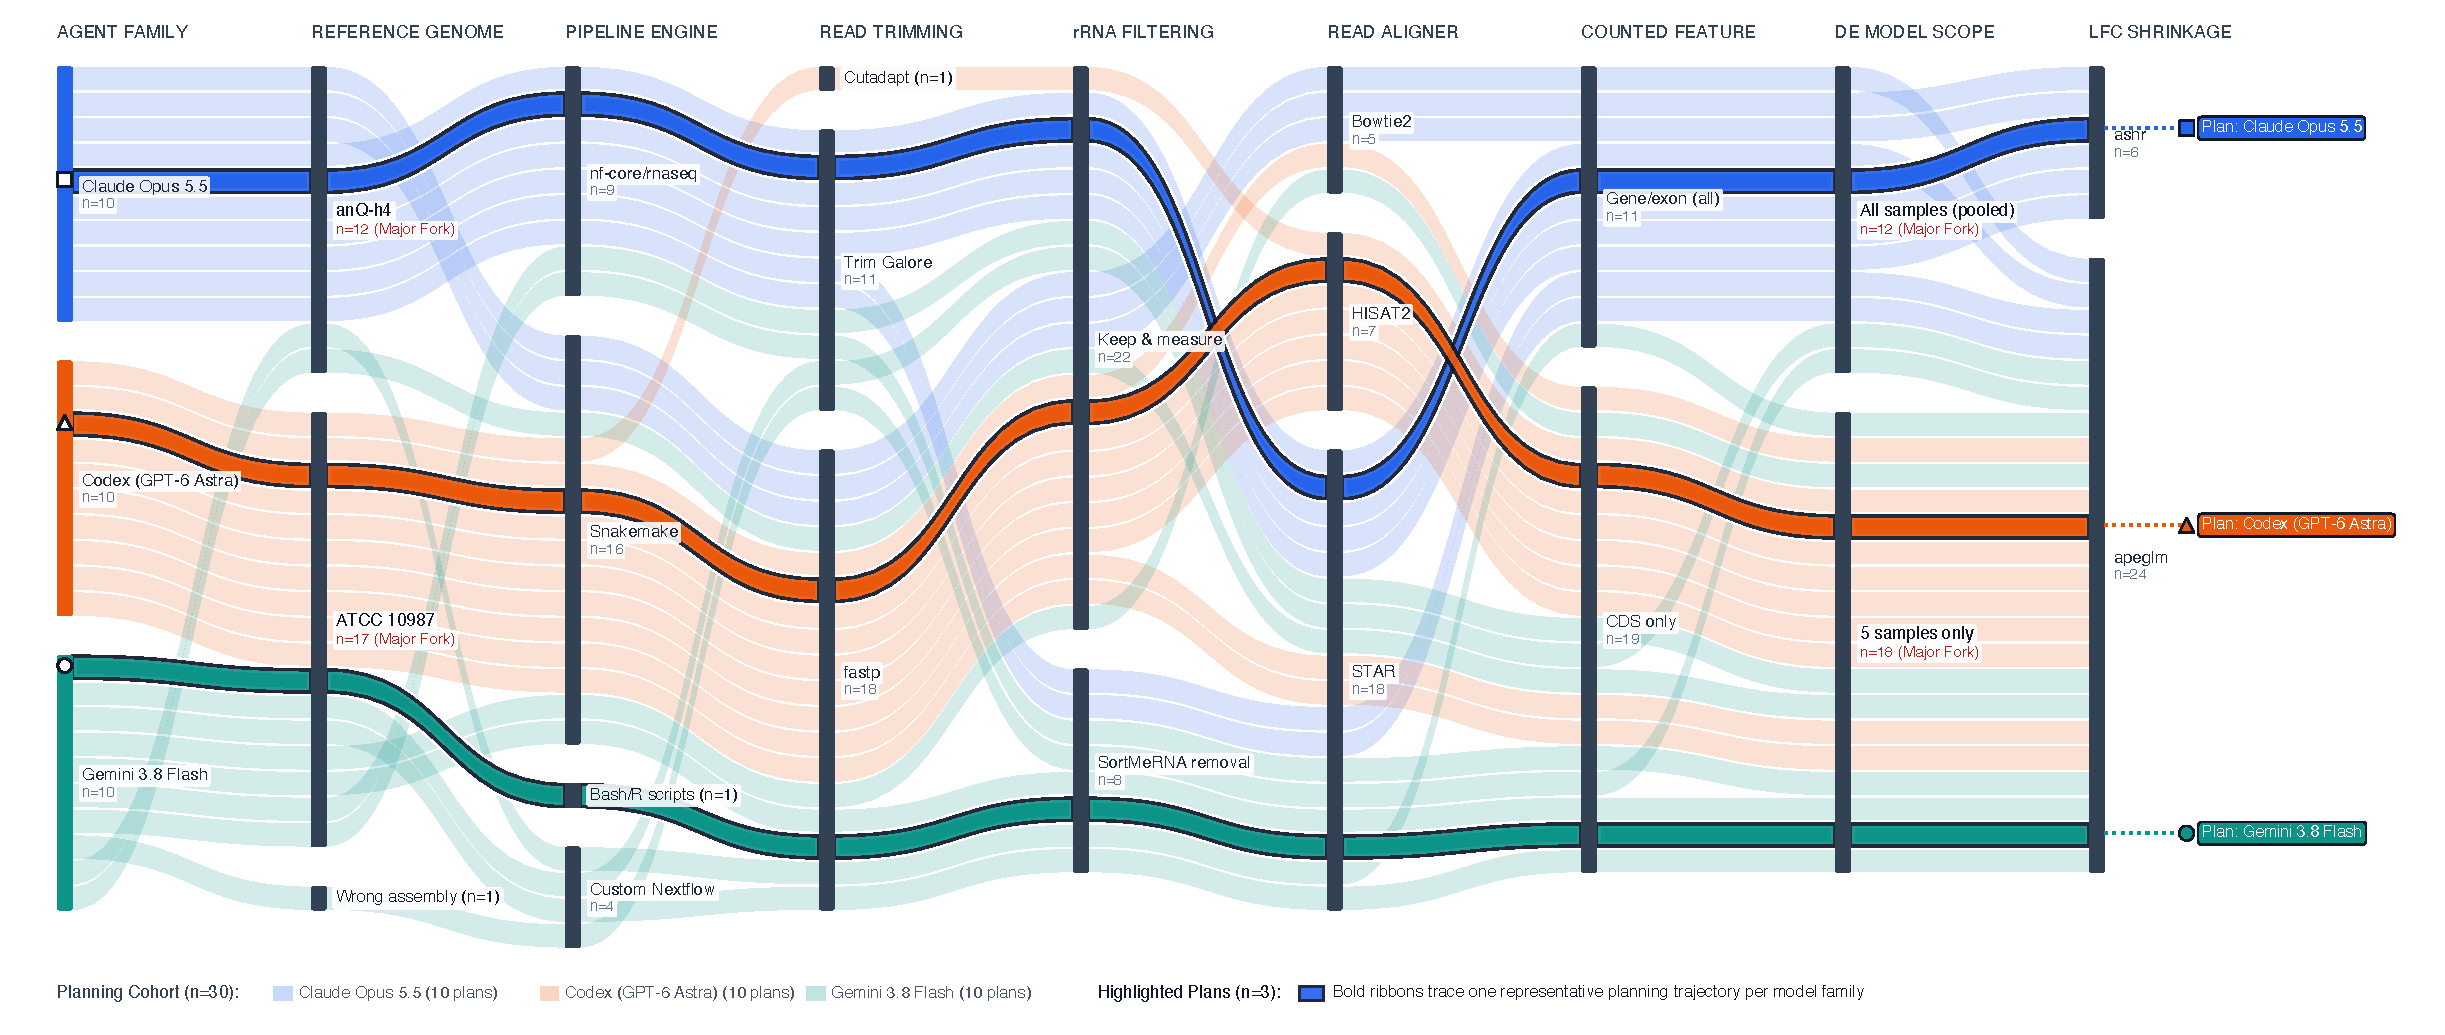
\includegraphics[width=0.90\textwidth]{figures/figure1_agent_trajectories.pdf}
\caption{\textbf{Thirty autonomous agents propose 18 different pipelines for the same bacterial RNA-seq study}.
Alluvial diagram tracing 30 independent reanalysis plans for a published \textit{Bacillus cereus} carbohydrate-supplementation study (PMC12804731) \cite{vyklicka2026} without access to Galaxy infrastructure. Plans were generated by 10 Anthropic Claude Code agents running Claude Opus 5.5 (blue), 10 OpenAI Codex agents running GPT-6 Astra (orange), and 10 Google Antigravity agents running Gemini 3.8 Flash (teal). Columns represent eight sequential pipeline decisions from reference assembly selection to log-fold-change shrinkage, with node heights proportional to the number of agents choosing each option ($n = 30$ total). Transparent ribbons show individual plans, while bold ribbons with geometric markers trace one executed trajectory per model family (square for Claude, triangle for Codex, and circle for Gemini). Across all eight steps, the 30 plans split into 18 distinct workflows (11 distinct designs across the five result-changing steps), and 29 of 30 differed from the published workflow.}
\label{fig:agent_trajectories}
\end{figure}

\subsection{... and leave a dusty trail of intermediates}

We then asked one agent per provider to actually execute its plan locally. Once execution began, each run drifted even further from its own plan as it improvised around local software and archive metadata (Supplementary Table~\ref{tab:agent_resources}). All three runs recovered headline repression of \textit{nheB} and induction of \textit{entFM} (Figure~\ref{fig:agent_execution}A), yet diverging reference genomes silently altered the detected toxin repertoire. Aligning to \textit{B.\ pacificus} anQ-h4 missed cytotoxin K (\textit{cytK2}) entirely because that assembly lacks the locus, whereas aligning to the sequenced isolate \textit{B.\ cereus} ATCC 10987 recovered active \textit{cytK2} transcription across every library (Figure~\ref{fig:agent_execution}B). Compute footprints varied by orders of magnitude, and the three runs left behind 26 unversioned glue scripts totaling over 1,200 lines of non-portable code (Supplementary Tables~\ref{tab:agent_resources} and~\ref{tab:agent_scripts}). Without shared infrastructure, local agents leave a debris field of disposable scripts in place of a verifiable record.

\begin{figure}[!htbp]
\centering
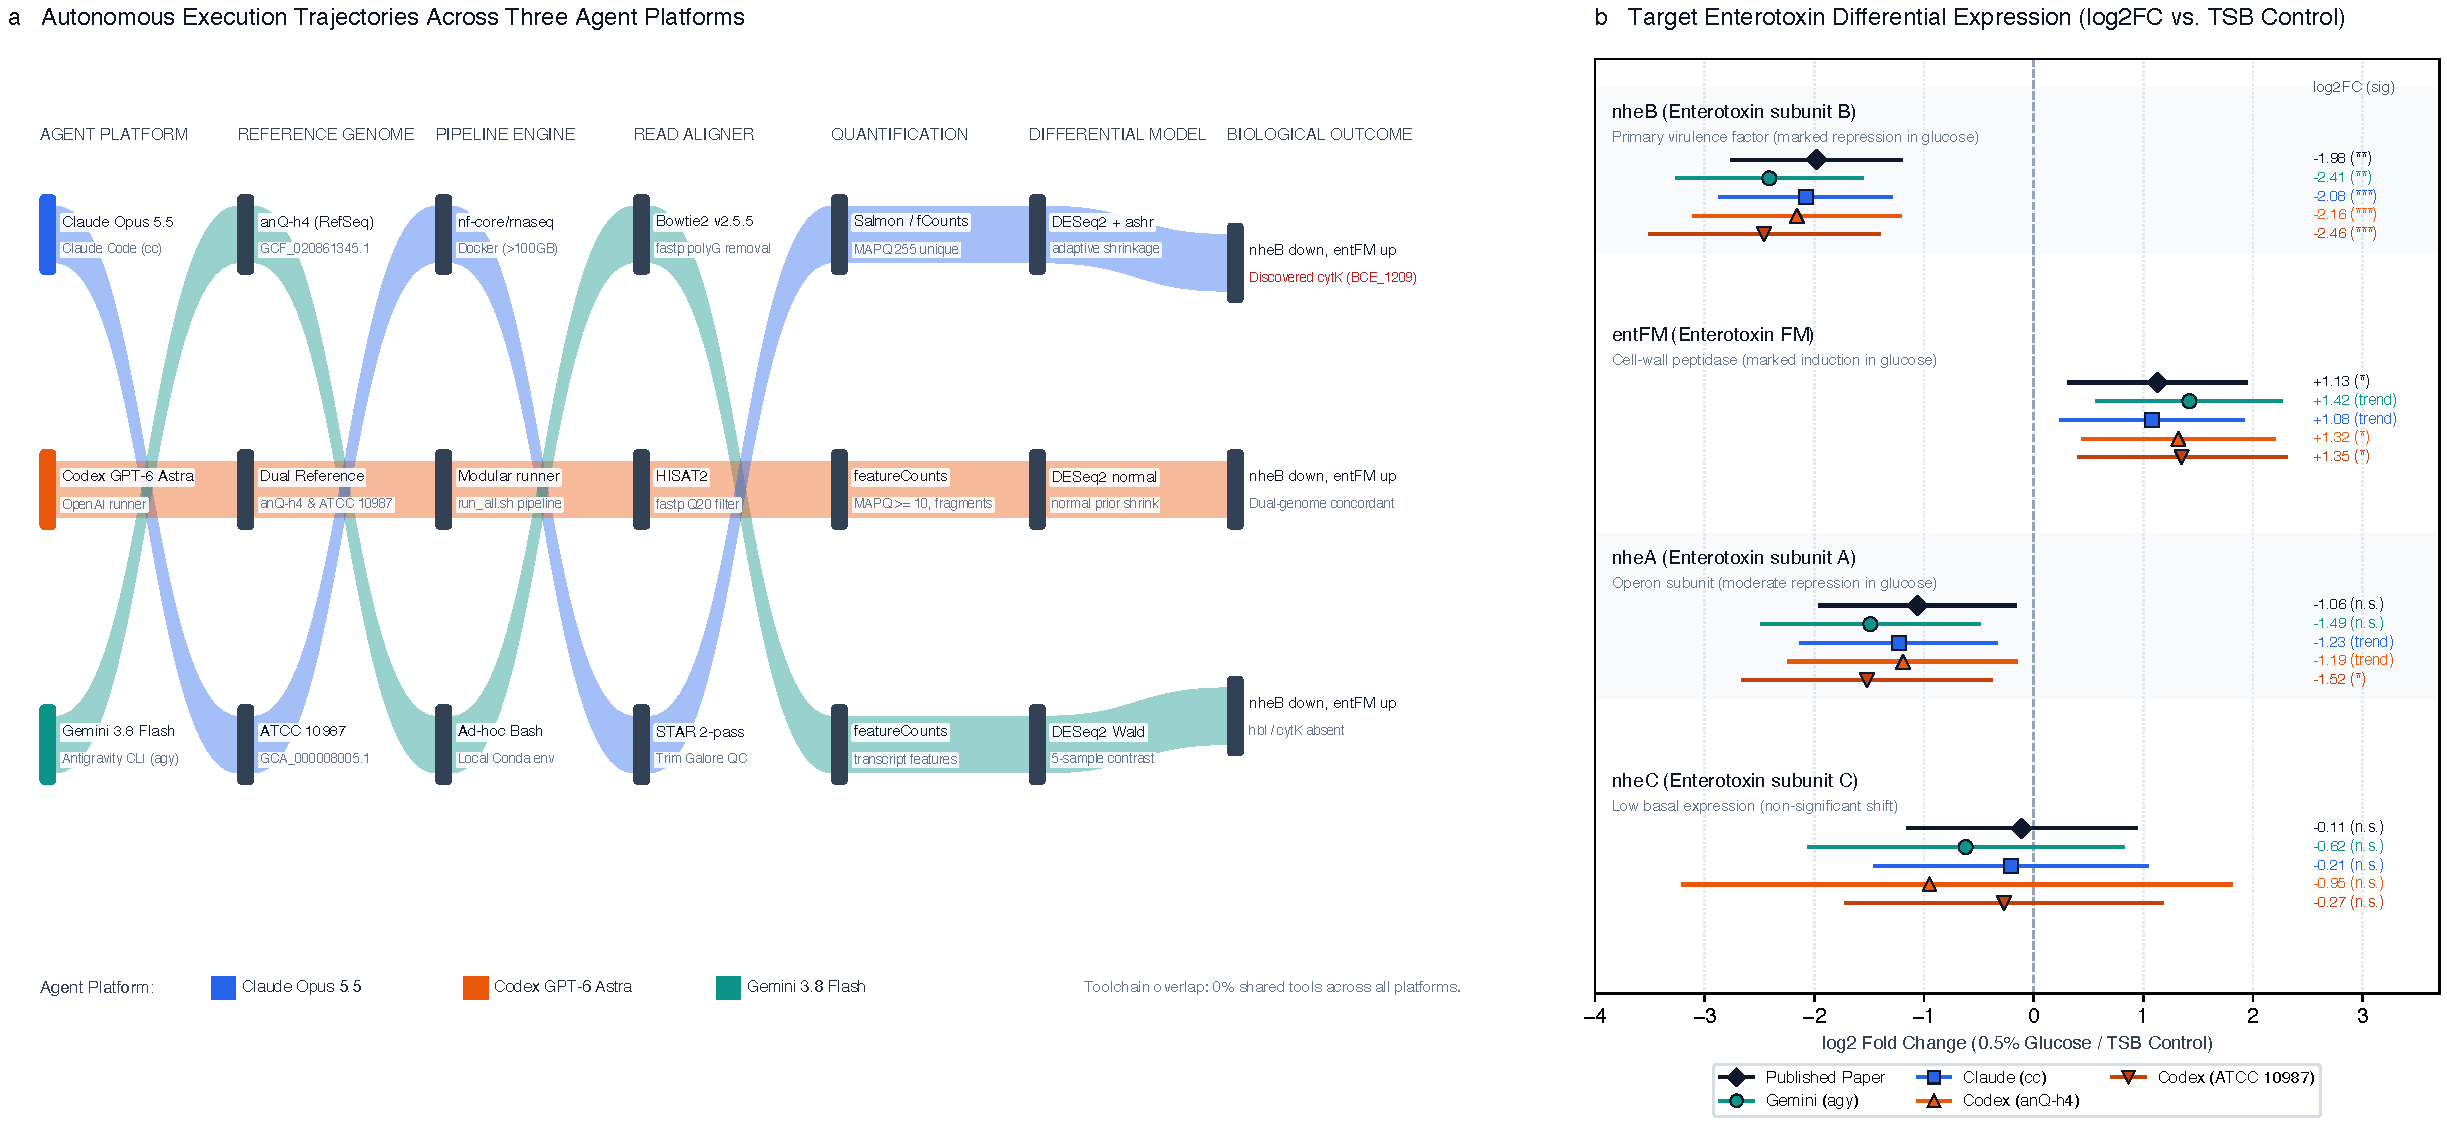
\includegraphics[width=\textwidth]{figures/figure2_agent_execution.pdf}
\caption{\textbf{Local agent runs recover headline enterotoxin signals but diverge on reference genomes and leave unversioned glue code.} 
\textbf{A}, Differential expression estimates ($\log_2\text{FC}$ with 95\% confidence intervals) and adjusted $p$-values for target enterotoxin genes (\textit{nheB}, \textit{entFM}, \textit{nheA}, \textit{nheC}, and \textit{cytK2}) compared against the published study (black diamonds, Vyklick{\'a} et al.\ \cite{vyklicka2026}). OpenAI Codex (orange and rust across two reference assemblies) and Google Gemini via Antigravity (teal) report unshrunken DESeq2 Wald estimates, whereas Claude Code (blue, \texttt{nf-core/differentialabundance}) reports \texttt{ashr}-shrunken estimates (for \textit{nheC} on \textit{B.\ pacificus}, where independent filtering sets $p_{\text{adj}}$ to \texttt{NA}, the unadjusted $p$-value is shown). All three agents confirmed strong repression of \textit{nheB} and induction of \textit{entFM}. 
\textbf{B}, Reference-assembly mismatch at the cytotoxin K (\textit{cytK2}) locus. Aligning against the sequenced isolate \textit{B.\ cereus} ATCC 10987 in Claude Code and Codex recovered active baseline \textit{cytK2} transcription across all libraries (548--1,420 read pairs per library, mean 797, DESeq2 $\text{baseMean} = 831$, $p_{\text{adj}} = 0.43$). Aligning against \textit{B.\ pacificus} anQ-h4 missed \textit{cytK2} entirely because that assembly lacks the locus.}
\label{fig:agent_execution}
\end{figure}

\clearpage
\subsection{Agentic science on public infrastructure: The Galactic plane}

Eliminating pipeline fragmentation, disposable glue code, and local hardware limits requires pairing domain skills with a shared execution engine (Figure~\ref{fig:architecture}). Any coding agent---or Orbit, our desktop workbench---connects to public Galaxy infrastructure \cite{galaxy2024} through modular skills and the Galaxy MCP server \cite{galaxymcp2026, galaxyskills2026}. Instead of improvising shell commands, the agent invokes containerized tools and peer-reviewed workflows via typed API calls across national supercomputers and cloud nodes (Figure~\ref{fig:architecture}, bottom), running everything from memory-intensive aligners like STAR \cite{dobin2013} to foundation models and petabyte-scale index searches---such as AlphaGenome \cite{alphagenome2025}, Logan \cite{logan2024}, and LexicMap \cite{lexicmap2025}---that no personal workstation can host.

\begin{figure}[!htbp]
\centering
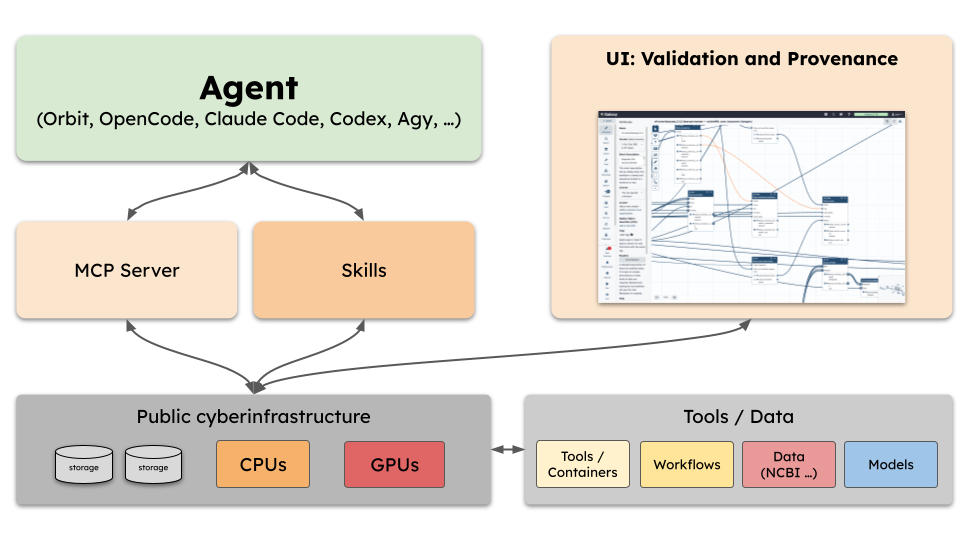
\includegraphics[width=0.95\textwidth]{figures/freiburg-oct20.png}
\caption{\textbf{Architecture for verifiable agentic science on public infrastructure.} 
\textbf{Agent} (top left): Researchers use Orbit or connect any generic coding agent (such as OpenCode, Claude Code, OpenAI Codex, or Antigravity CLI). 
\textbf{MCP Server and Skills} (middle left): Curated domain skills supply validated bioinformatics protocols, while the Galaxy MCP server translates agent actions into typed API calls in place of unconstrained shell commands. 
\textbf{UI: Validation and Provenance} (top right): Galaxy's visual workflow editor and history interface provide pre-execution schema validation and an inspectable provenance record for human steering and verification. 
\textbf{Public cyberinfrastructure and Tools/Data} (bottom): Galaxy schedules containerized tools, peer-reviewed workflows, public datasets (NCBI, ENA, BRC-Analytics), and large models across CPU, GPU, and storage allocations on national supercomputing infrastructure.}
\label{fig:architecture}
\end{figure}

Shared infrastructure makes complete provenance mandatory by default (Figure~\ref{fig:architecture}, top right). Narrative model summaries omit silent parameter changes and failed retries, and few biologists possess version control discipline over interactive shell sessions. Pushing execution onto Galaxy and Orbit records every input file, tool version, parameter, and intermediate dataset in a durable, shareable Galaxy history and workflow graph. The research notebook then links each narrative claim directly to the corresponding Galaxy datasets and job invocations, making the entire analysis human-readable and immediately verifiable. When an analysis needs custom code, the agent registers that script as a versioned, containerized User-Defined Tool\footnote{Because executing arbitrary user-supplied tool definitions on public supercomputing infrastructure carries security and resource risks, User-Defined Tool registration currently requires account approval on UseGalaxy.org or routes through an automated packaging and review pipeline on UseGalaxy.eu (see Discussion).} inside the workflow rather than leaving an untracked local file.

\subsection{Reproducing a paper using a generic agent on the Galactic plane}

To test how shared infrastructure changes interactive analysis, we connected Google's Antigravity CLI (Gemini 3.8 Flash) to UseGalaxy.org via the Galaxy MCP server \cite{galaxymcp2026} to reproduce the \textit{B.\ cereus} RNA-seq study \cite{vyklicka2026} in a human-in-the-loop session. Unlike local runs that generated 26 unversioned scripts or exhausted laptop disk space, the entire replication ran on free public supercomputers (Figure~\ref{fig:bacillus_replication}).

Visual workflow provenance proved essential before a single job launched. Both the local GPT-6 Astra run and the MCP-connected Gemini 3.8 Flash agent initially selected HISAT2, a eukaryotic spliced aligner that is inappropriate for an intronless bacterium (see Methods). Quantifying reads against bacterial coding sequences with Kallisto \cite{bray2016near} avoids spurious split-read mappings and finishes each library in 38--60~seconds instead of minutes to hours, provided split frameshift CDS headers are resolved (see Methods). While domain skills can encode prokaryotic tool preferences for local and remote agents alike, Galaxy renders the proposed pipeline as a visual workflow graph before execution, allowing us to spot HISAT2 at a glance and steer the agent to Kallisto (with both aligners yielding concordant fold changes, $r = 0.9622$).

Formal workflow validation also prevented silent scripting hacks. Whereas a local pilot run deduplicates split bacterial CDS headers via a throwaway script on disk, Galaxy records header deduplication as an explicit history step. Galaxy's workflow engine also validates collection types before jobs launch: when the agent wired an incompatible standalone \texttt{tximport} step between Kallisto's output collection and DESeq2, the editor flagged the mismatch in orange so the agent routed the transcript-to-gene map into DESeq2's built-in \texttt{tximport} mode up front (Figure~\ref{fig:bacillus_replication}A,B). The validated workflow reproduced fivefold repression of \textit{nheB} ($p_{\text{adj}} = 2.99 \times 10^{-3}$), nearly threefold repression of \textit{nheA} and induction of \textit{entFM}, and unchanged \textit{nheC} expression (Figure~\ref{fig:bacillus_replication}D, see Methods). Auditing the resulting Galaxy Page notebook (Figure~\ref{fig:bacillus_replication}C) against the history confirmed that every embedded dataset card and fold-change summary resolves to verified history outputs (Supplementary Table~\ref{tab:brc_artifacts}).

\begin{figure}[!htbp]
\centering
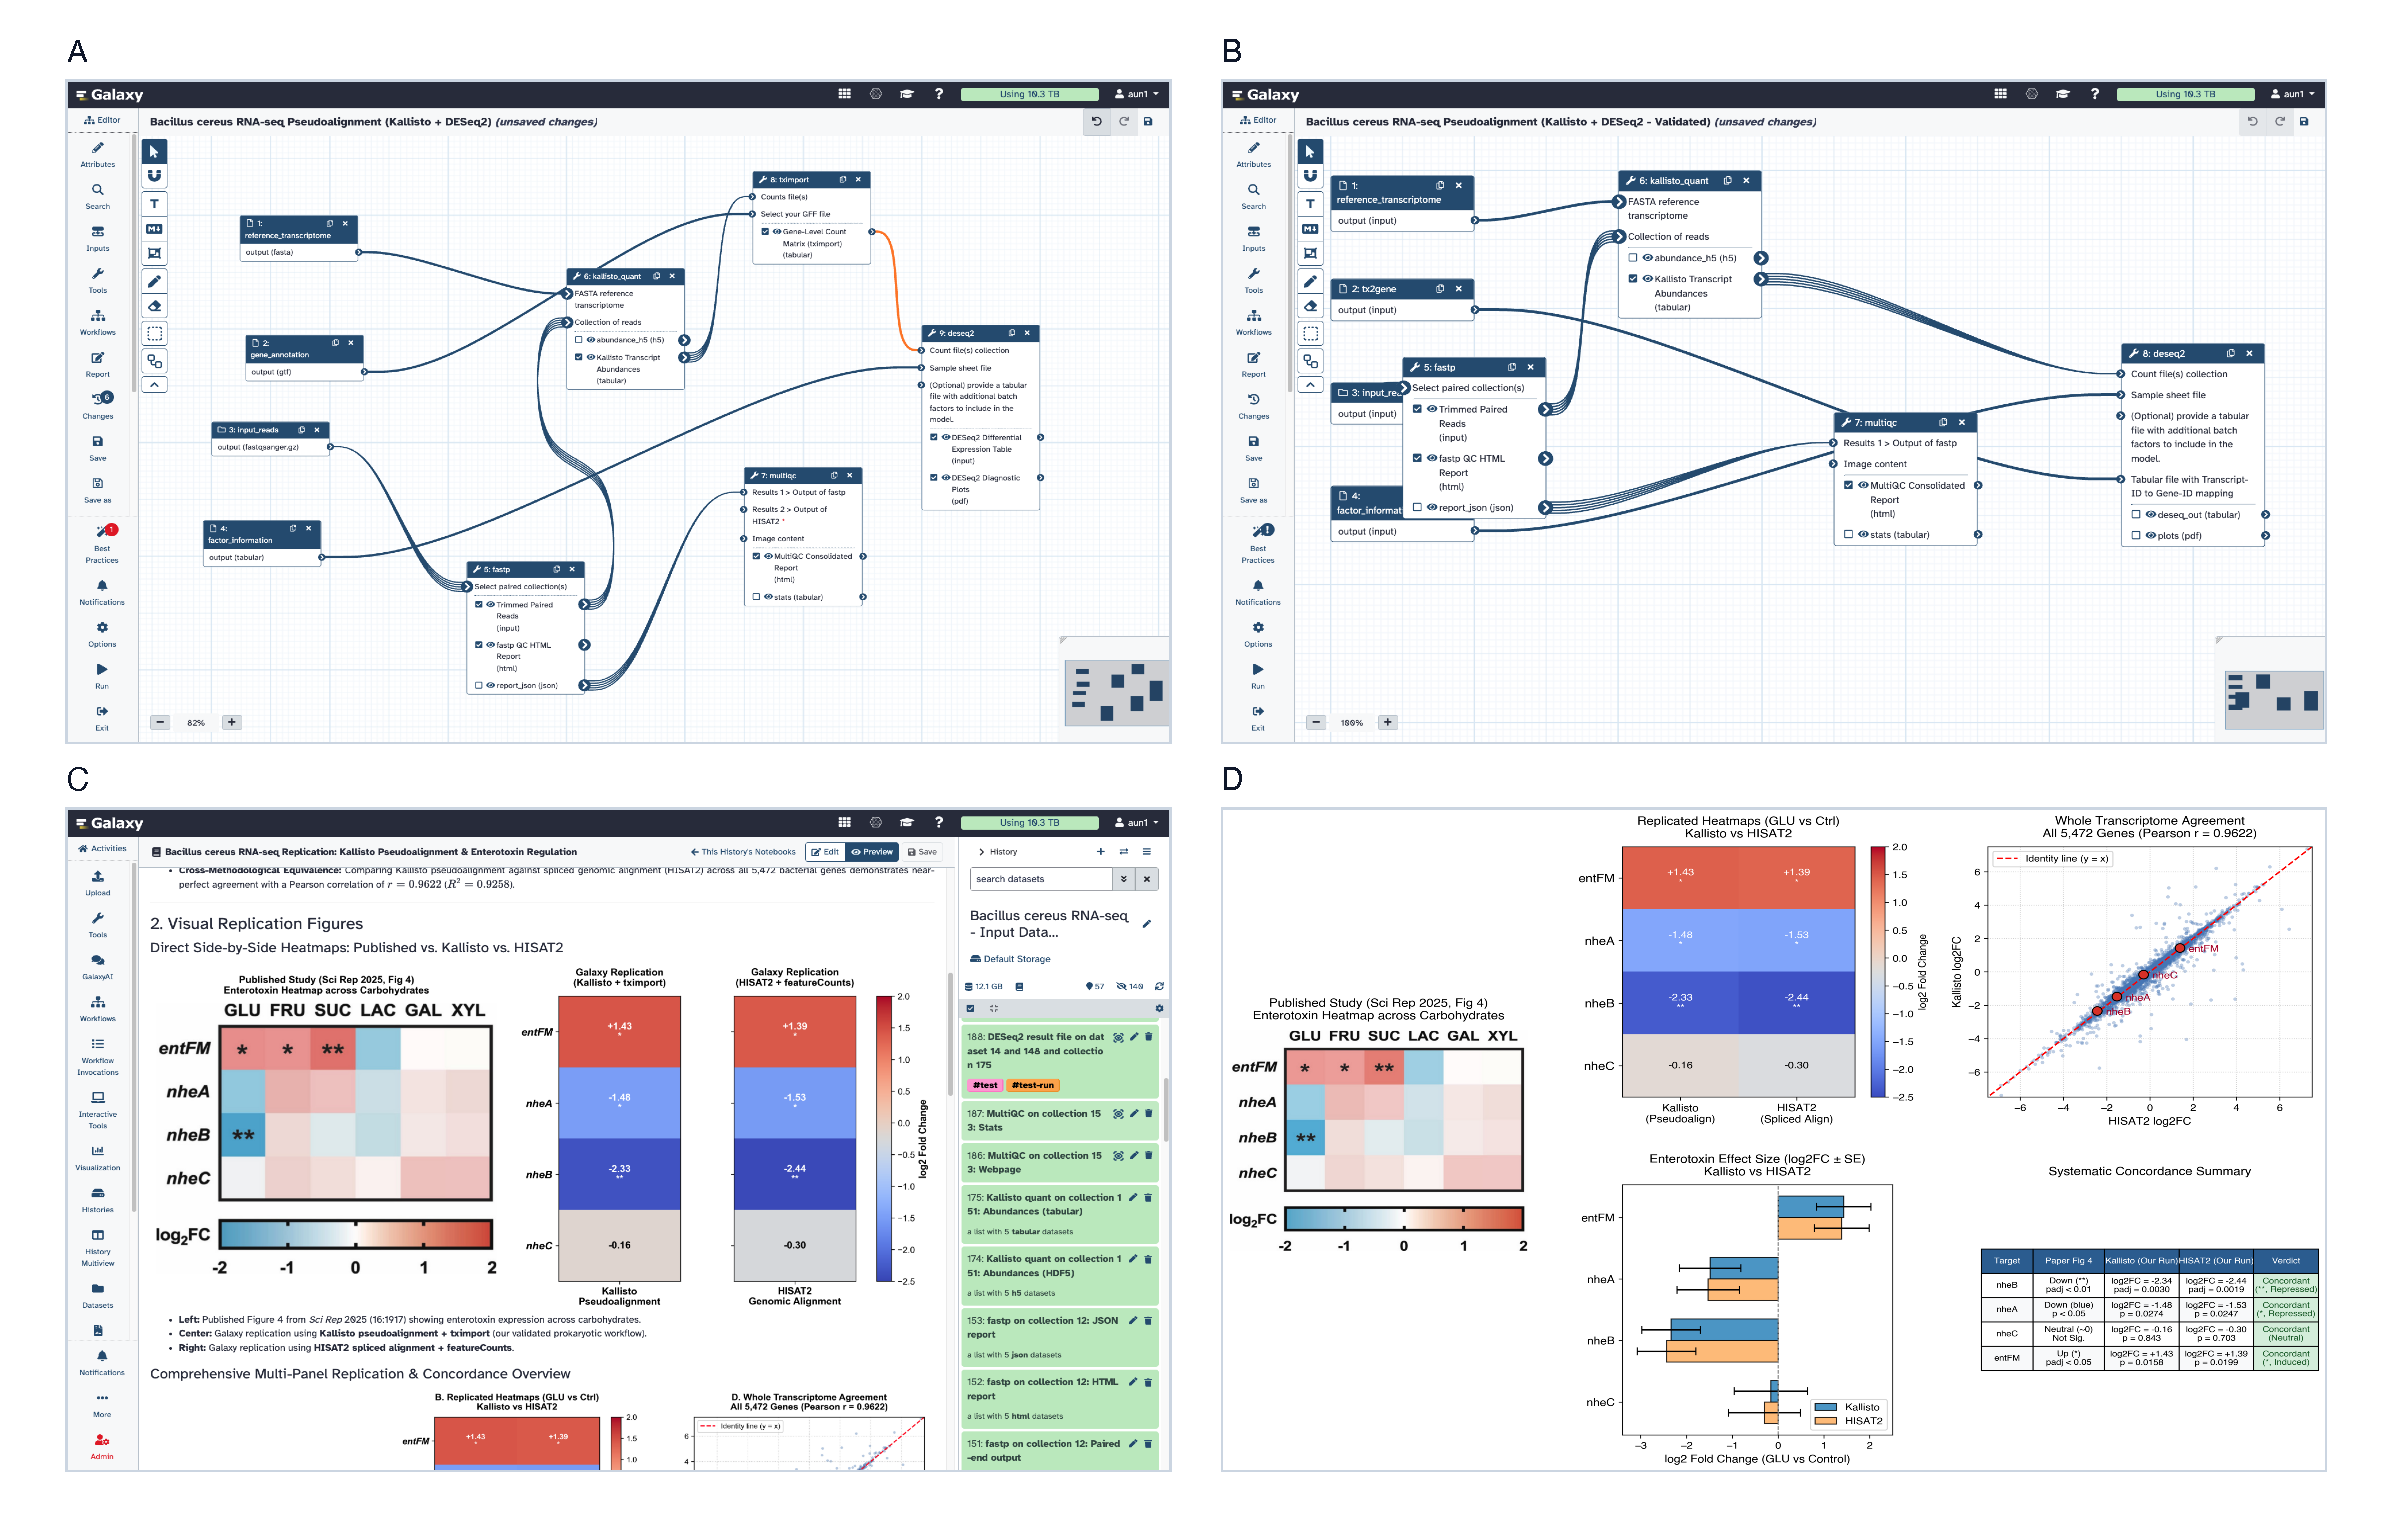
\includegraphics[width=\textwidth]{figures/figure_bacillus_replication.pdf}
\caption{\textbf{Workflow and execution provenance on free public infrastructure catches pipeline errors and reproduces bacterial RNA-seq profiles.} 
\textbf{A}, Pre-execution workflow validation on UseGalaxy.org. When an agent connected via the Galaxy MCP server inserts an incompatible standalone \texttt{tximport} step between a Kallisto output collection and DESeq2, the workflow editor flags the type mismatch in orange before any jobs launch. 
\textbf{B}, Validated workflow after autonomous repair. Passing the transcript-to-gene table (\texttt{tx2gene.tsv}) to DESeq2's built-in \texttt{tximport} mode resolves all workflow connections in green. 
\textbf{C}, Live provenance and interactive Galaxy History Notebook. Jobs execute on free public ACCESS-CI supercomputing allocations while completed datasets populate the right-hand history panel and the center notebook links narrative text to verified history dataset IDs. 
\textbf{D}, Biological replication of Vyklick{\'a} et al.\ \cite{vyklicka2026} across the \textit{B.\ cereus} ATCC 10987 coding transcriptome. Glucose supplementation represses enterotoxin subunits \textit{nheB} (5.05-fold down, $\log_2\text{FC} = -2.335$, $p_{\text{adj}} = 2.99 \times 10^{-3}$) and \textit{nheA} (2.80-fold down, $\log_2\text{FC} = -1.484$, raw $p = 0.0274$, $p_{\text{adj}} = 0.106$), leaves regulatory subunit \textit{nheC} unchanged ($\log_2\text{FC} = -0.158$, $p_{\text{adj}} = 0.907$), and induces \textit{entFM} (2.70-fold up, $\log_2\text{FC} = +1.432$, raw $p = 0.0158$, $p_{\text{adj}} = 0.0730$). Across all 5,250 expressed coding loci (of 5,472 total), Kallisto pseudoalignment and HISAT2 alignment agree closely (Pearson $r = 0.9622$, $R^2 = 0.9257$).}
\label{fig:bacillus_replication}
\end{figure}

\subsection{An opinionated agent}

Domain skills and the Galaxy MCP server guide generic command-line agents effectively, yet terminal agents require command-line fluency and nothing in a skill file stops an agent from falling back on untracked local shell commands when a step fails. To give bench biologists a friendly desktop application whose harness can block and record what the agent does, we built Orbit on top of Pi.dev (Figure~\ref{fig:architecture}). Orbit is Galaxy-first, steering tool execution to Galaxy while keeping guarded local execution for lightweight work, tracking live cluster jobs, registering custom scripts as versioned User-Defined Tools \cite{galaxyudt2026}, and syncing the analysis record into a version-controlled project notebook across commercial, public API, and local open-weight models (Table~\ref{tab:validation_summary}).

Controlling an agent operates across three levels: domain skills that advise how to design an analysis, the MCP server that exposes typed Galaxy tools, and harness logic that mediates every tool call in code. Harness logic is essential because prompt-level instructions can be ignored. Because Galaxy provides a server-side record of typed tool runs that the agent cannot edit, Orbit's harness logic can verify directly against Galaxy whether a step's job has actually finished before allowing the plan step to be marked complete (see Methods). These guarantees apply to the record rather than the science: Orbit does not make an agent's analytical choices correct, but its harness logic ensures that what the agent did is checkable.

\begin{table}[!htbp]
\centering
\scriptsize
\setlength{\tabcolsep}{4.5pt}
\renewcommand{\arraystretch}{1.18}
\begin{tabularx}{\textwidth}{p{2.9cm}p{2.3cm}p{2.3cm}X}
\toprule
\textbf{Analysis \& System} & \textbf{Assay \& Scale} & \textbf{Agent \& Stack} & \textbf{Highlight} \\
\midrule
\textbf{\textit{Bacillus cereus} enterotoxin regulation} \newline Vyklick{\'a} et al.\ \cite{vyklicka2026} & Bacterial RNA-seq \newline (5 libraries, 5,472 coding loci) & Generic CLI agent + Galaxy MCP + Skills & Replaces 26 unversioned local glue scripts from unconstrained runs with one validated workflow, catching split bacterial CDS annotations on a pilot run and switching to $\sim 5\times$ faster prokaryotic pseudoalignment (38--60~s per library). \\
\addlinespace[0.35em]
\textbf{Mouse cortex spatial transcriptomics} \newline Miao et al.\ \cite{miao2026}, Sun et al.\ \cite{sun2024} & Mammalian scRNA-seq + spatial prediction \newline (3,405 spatial \& 5,613 reference cells) & Orbit + 2 UDTs on UseGalaxy.org & Reconciles an undocumented 1,000-cell tutorial subset in Extended Data Fig.\ 1c against the cited 5,613-cell Dataset 15 archive, reproduces the tutorial subset on Galaxy, and scales to all 5,613 reference cells to triple prediction accuracy ($r = 0.0861$ to $0.2553$). \\
\addlinespace[0.35em]
\textbf{\textit{Aspergillus fumigatus} azole time-course} \newline Hokken et al.\ \cite{hokken2018} & Fungal RNA-seq \newline (30 libraries, 3 isolates $\times$ 5 timepoints) & Orbit + Workflow Foundry + BRC-Analytics + 3 UDTs & Compiles a 60-step workflow from published methods text, uncovers that the authors fitted one pooled 30-sample model instead of pairwise contrasts, and replaces a defunct web service and two interactive browser tools with automated UDTs. \\
\addlinespace[0.35em]
\textbf{\textit{Anopheles gambiae} infection chromatin} \newline Ruiz et al.\ \cite{ruiz2021} & Vector ATAC-seq \newline (midguts \& salivary glands, 4 libraries) & Orbit + 3 UDTs on UseGalaxy.org & Reproduces 90.7--93.2\% of published chromatin peaks without free parameters, while showing that the paper's headline region counts reflect unmerged per-replicate table rows and custom overlap filtering. \\
\addlinespace[0.35em]
\textbf{\textit{Aedes aegypti} midgut single-cell atlas} \newline Wang et al.\ \cite{wang2024} & Vector 10x 3' scRNA-seq \newline (2 replicates, 6,707 post-QC cells) & Orbit + BRC-Analytics on UseGalaxy.org & Stages non-model vector reference data into a public single-cell pipeline, fixes a mitochondrial gene prefix mismatch that breaks generic QC, and recovers published cell-type markers de novo. \\
\addlinespace[0.35em]
\textbf{\textit{Plasmodium vivax} VIR phylogenomics} \newline Carlton et al.\ \cite{carlton2008}, Harrison et al.\ \cite{harrison2020} & Structure-aware phylogenomics \newline (3 genomes, 2,592 proteins) & Orbit + 10 UDTs (1 GPU, 9 CPU) on UseGalaxy.org & Orchestrates GPU protein structure models (ProstT5, Foldseek, and FoldMason) via unprivileged UDTs, collapsing 146 sequence-fragmented antigen subfamilies into 73--76 structural classes and showing that over 97\% of proteins belong to folds shared across three continents. \\
\addlinespace[0.35em]
\textbf{Pathogen emergence dating across 42 cohorts} \newline 42 BEAST alignments across 37 studies \cite{gire2014genomic, dudas2017virus, hill2019skygrid, faria2021genomics, pond2026hyphaeon} & Genomic epidemiology \newline (42 viral \& bacterial epidemic alignments, 41 unique) & Orbit + 2 UDTs on UseGalaxy.org & Dates 42 pathogen epidemic alignments in seconds per cohort instead of hours to days of Bayesian MCMC sampling, matching reference Bayesian emergence dates across 61.5--64.1\% of scored cohorts. \\
\bottomrule
\end{tabularx}
\caption{\textbf{Summary of empirical validations and discovery analyses executed on the Galactic plane.} Across seven biological investigations spanning bacteria, mammalian cortex, fungi, mosquito vectors, protozoan parasites, and 42 viral and bacterial epidemic alignments (41 distinct outbreaks across 37 publications), autonomous agents executed reproducible workflows on free public UseGalaxy.org and ACCESS-CI supercomputing infrastructure. Every analysis produced inspectable Galaxy histories, reusable workflows, and shareable research notebooks (complete accession identifiers in Supplementary Tables~\ref{tab:brc_artifacts}--\ref{tab:case3_artifacts}).}
\label{tab:validation_summary}
\end{table}

\subsection{From papers to skills: A spatial transcriptomics example}

Because imaging-based spatial transcriptomics measures only a few dozen genes across a tissue section, TISSUE \cite{sun2024} uses paired single-cell RNA-seq reference atlases to impute unmeasured transcripts and calibrate uncertainty intervals. Recently, Miao et al.\ \cite{miao2026} showcased Paper2Agent by wrapping TISSUE into an agent to predict expression and uncertainty for the vascular smooth muscle marker \textit{Acta2} across 3,405 mouse somatosensory cortex cells (33-gene osmFISH assay). Wrapping code into a standalone agent, however, leaves execution unverified unless input datasets and workflow steps are recorded on shared infrastructure.

Tasked with reproducing the Paper2Agent spatial benchmark, Orbit uncovered an ironic discrepancy: a benchmark designed to demonstrate automated agent reproducibility had silently run on a toy tutorial file rather than the full reference atlas it cited. Although Miao et al.\ \cite{miao2026} cited the 5,613-cell mouse cortex reference archive (Zenodo Dataset 15) in their Data Availability statement, Orbit's provenance audit revealed that Extended Data Figure 1c was generated from a 1,000-cell tutorial file (\texttt{tests/data/scRNA\_count.txt}) bundled inside the TISSUE repository, omitting 82\% of the cited reference cells and leaving predicted \textit{Acta2} expression nearly uncorrelated with ground truth ($r = 0.0861$, see Methods). Orbit registered two TISSUE User-Defined Tools on UseGalaxy.org, reproduced the 1,000-cell tutorial predictions to floating-point precision ($r = 1.0000$, $\Delta_{\max} < 10^{-15}$, $86.46\%$ Galaxy vs.\ $86.49\%$ local coverage at nominal 77\%, Figure~\ref{fig:spatial_comparison}A,B), and then scaled the workflow to all 5,613 reference cells in Dataset 15, tripling \textit{Acta2} prediction correlation to $r = 0.2553$ ($r = 0.2845$ in 33-gene cross-validation, $85.61\%$ coverage, Supplementary Table~\ref{tab:case1_artifacts}). Dataset and workflow provenance on public infrastructure immediately exposed a fivefold reference-data loss that had escaped unrecorded local execution.

\begin{figure}[!htbp]
\centering
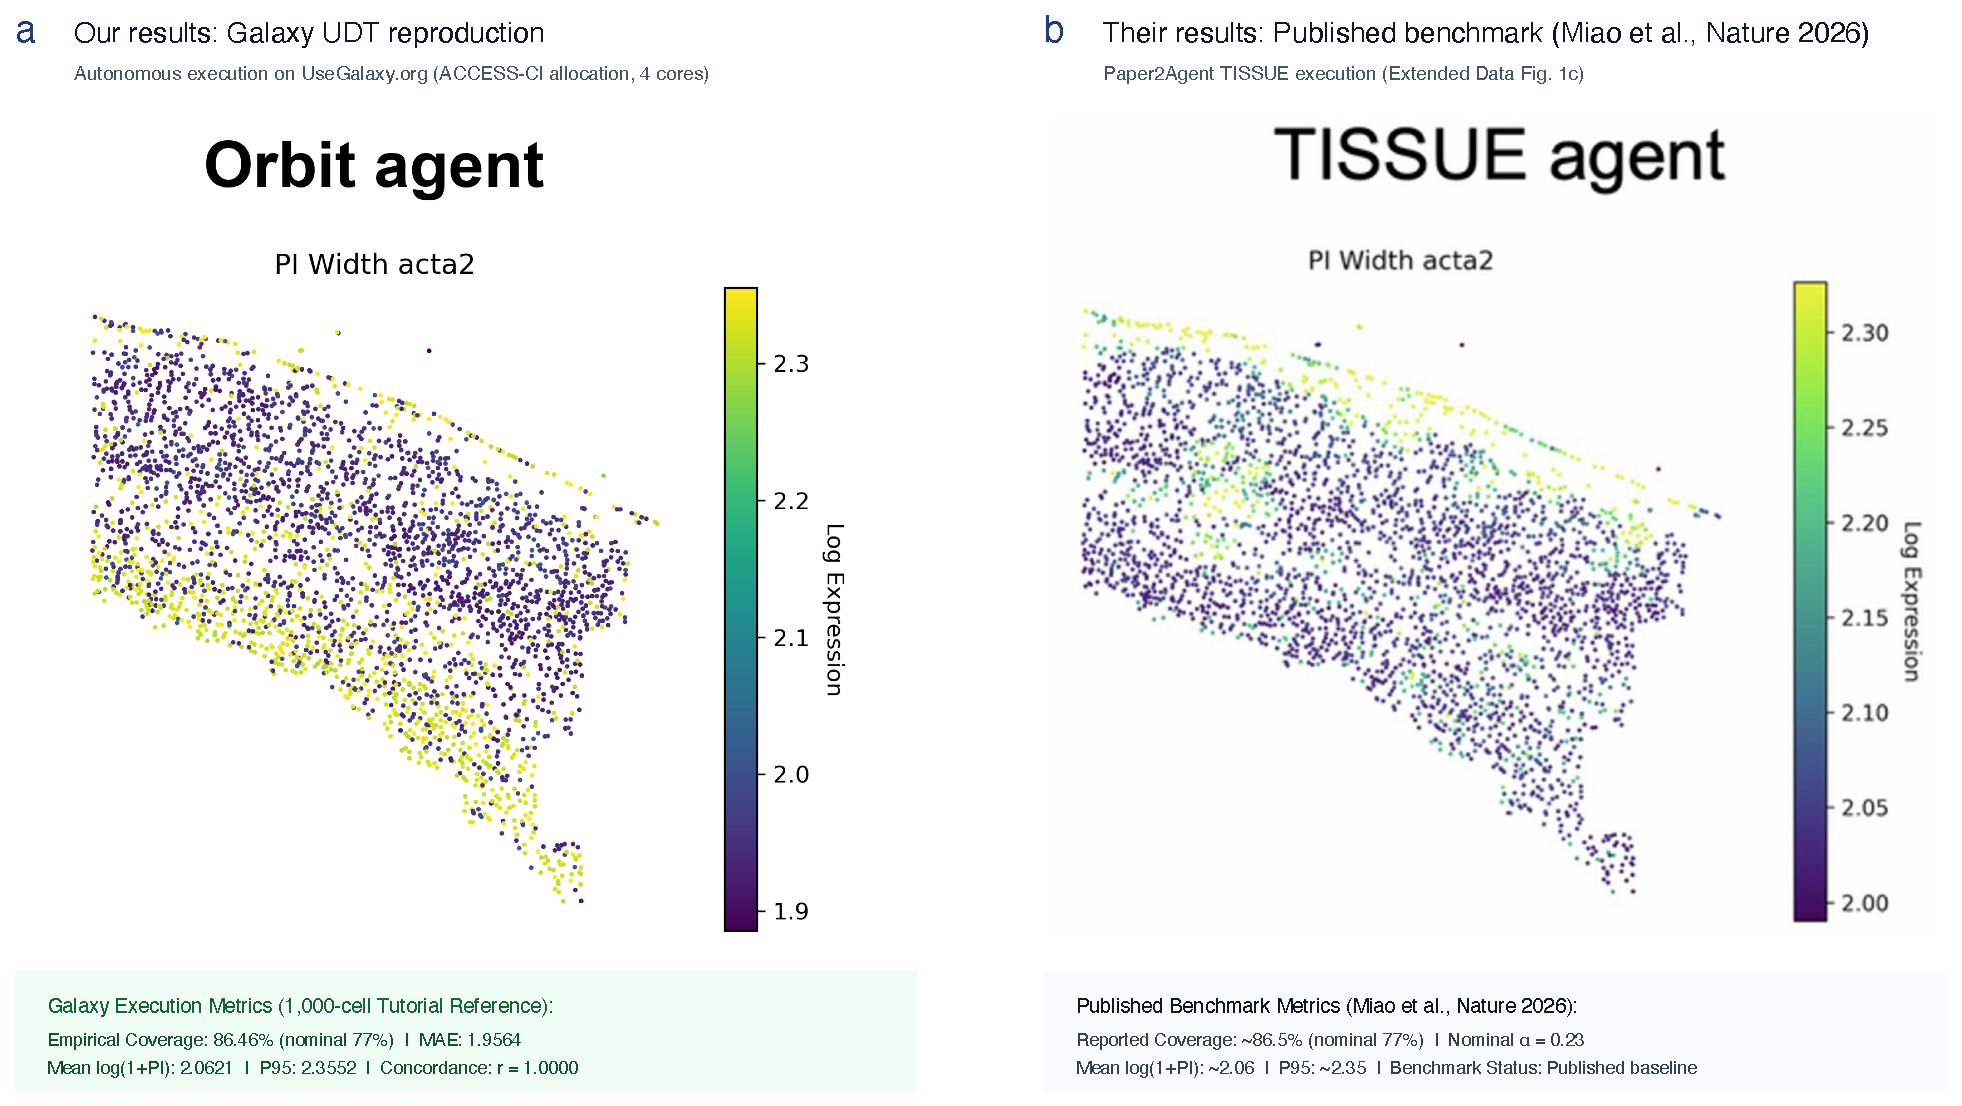
\includegraphics[width=0.88\textwidth]{figures/figure2_spatial_comparison.pdf}
\caption{\textbf{Reproducing and scaling a published spatial transcriptomics benchmark on public infrastructure.} 
\textbf{A}, Spatial map of conformal prediction interval (PI) widths ($\log(1 + \text{PI Width})$) for imputed \textit{Acta2} expression across 3,405 mouse somatosensory cortex cells, generated by Orbit via an unprivileged User-Defined Tool (\texttt{tissue\_spatial\_prediction}) on UseGalaxy.org using the 1,000-cell tutorial reference subset. Point predictions on Galaxy matched local execution to floating-point precision ($r = 1.0000$, $\Delta_{\max} < 10^{-15}$), with 86.46\% empirical coverage on Galaxy (86.49\% locally) at the nominal 77\% threshold ($\alpha = 0.23$) and mean $\log(1 + \text{PI Width})$ of 2.0621 (2.0634 locally). 
\textbf{B}, Published Paper2Agent benchmark from Extended Data Figure 1c of Miao et al.\ \cite{miao2026} on the same 1,000-cell tutorial subset (nominal $\alpha = 0.23$). Stochastic $k$-means cell-variability grouping shifts individual high-uncertainty cells between the ventral boundary and the pial edge, while both runs capture the same overall uncertainty range ($\sim 1.89\text{--}2.35$ vs.\ $2.00\text{--}2.32$).}
\label{fig:spatial_comparison}
\end{figure}

\subsection{Uncovering analysis inconsistencies and defunct tools}

To test multi-step functional genomics, we combined Orbit with Workflow Foundry \cite{foundry2026}---which compiles published methods prose into validated Galaxy workflows---and BRC-Analytics \cite{brcanalytics2026}, which stages curated pathogen reference assemblies and sequencing archives (see Methods). We reconstructed the 30-sample RNA-seq study of Hokken et al.\ \cite{hokken2018} in \textit{Aspergillus fumigatus}, an airborne mold causing lethal invasive infections where frontline triazole resistance is rising. Hokken et al.\ profiled transcriptional responses to itraconazole across three clinical isolates and five exposure timepoints in duplicate (PRJNA482512). BRC-Analytics staged the Af293 genome and all 30 libraries, and Workflow Foundry compiled a 60-step Galaxy workflow (86.88\% mean unique alignment vs.\ 86.5\% published, see Methods).

Comparing our initial differential expression outputs against the published tables uncovered an unstated statistical modeling choice and two broken downstream tools. Four separate 12-sample pairwise DESeq2 models reproduced the published fold changes ($r \ge 0.999$) but missed up to 39\% of reported differentially expressed genes at later timepoints. Auditing the supplementary spreadsheet revealed the forensic signature: every gene carried a single identical \texttt{baseMean} value across all four contrasts, proving the authors had fitted one pooled 30-sample model across all five timepoints simultaneously. With only two replicates per group, pooling all 30 libraries provides 25 residual degrees of freedom to stabilize dispersion and applies a uniform expression threshold ($\text{baseMean} \ge 30$)---yet leaving that choice unstated causes a pairwise reproduction to lose nearly 40\% of the signal. Switching our Galaxy workflow to a pooled 30-sample model reproduced the published standard errors to four decimal places and matched DEG counts within 0.3--1.3\% at every timepoint ($r = 0.9996\text{--}0.9999$, Figure~\ref{fig:brc_reproductions}A), while three User-Defined Tools replaced a decommissioned fungal Gene Ontology server (AspGD) and an interactive browser utility (REVIGO) to recover the shift from cell-wall stress to drug-efflux induction (Supplementary Table~\ref{tab:brc_artifacts}).

\begin{figure}[!htbp]
\centering
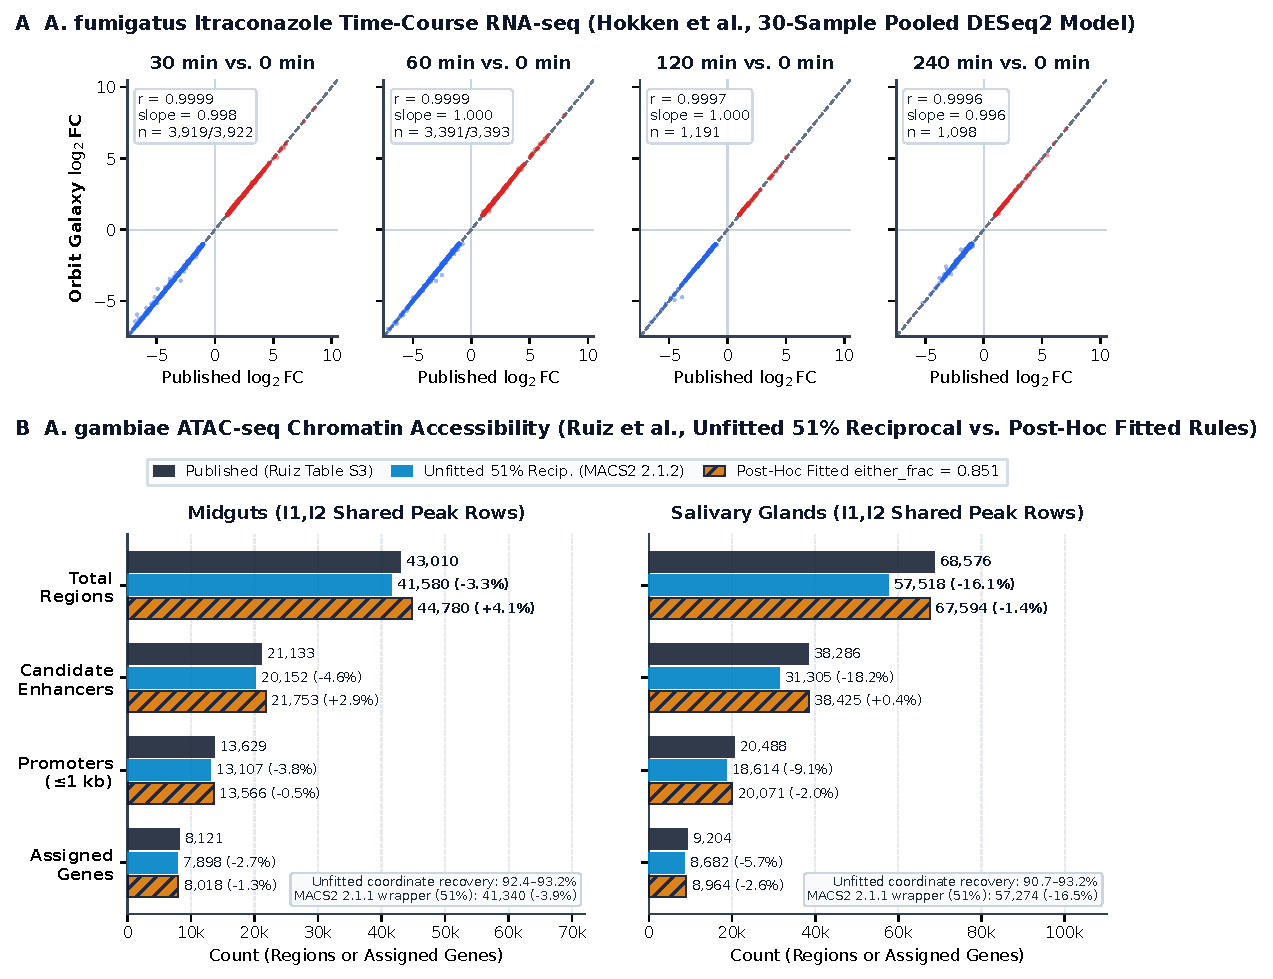
\includegraphics[width=\textwidth]{figures/figure_brc_reproductions.pdf}
\caption{\textbf{Reproducing pathogen and vector functional genomics studies on UseGalaxy.org.} 
\textbf{A}, Transcriptomic response of the pathogenic mold \textit{Aspergillus fumigatus} to the antifungal drug itraconazole across 30 libraries (Hokken et al.\ \cite{hokken2018}). A pooled 30-sample DESeq2 model compiled via Workflow Foundry reproduces published $\log_2$ fold changes across all four post-exposure timepoints ($r = 0.9996\text{--}0.9999$, slopes $0.996\text{--}1.000$). Published differentially expressed gene counts match within 0.3--1.3\% ($n = 3,919$ of $3,922$ at 30 min, $3,391$ of $3,393$ at 60 min, $1,191$ at 120 min, and $1,098$ at 240 min). 
\textbf{B}, Chromatin accessibility in \textit{Anopheles gambiae} malaria mosquito midguts and salivary glands during \textit{Plasmodium falciparum} infection (Ruiz et al.\ \cite{ruiz2021}). Unfitted MACS2 peak calling recovers 90.7--93.2\% of the authors' deposited genomic regions across all four libraries. Provenance-tracked overlap rules show how unmerged per-replicate rows and overlap filtering account for the paper's headline counts within 0.4--4.6\%.}
\label{fig:brc_reproductions}
\end{figure}

\subsection{Uncovering undocumented analysis details}

End-to-end provenance also separates reproducible chromatin biology from undocumented table formatting. In the ATAC-seq study of Ruiz et al.\ \cite{ruiz2021} across midguts and salivary glands of the malaria vector \textit{Anopheles gambiae}---the two epithelial barriers traversed by \textit{Plasmodium falciparum} parasites during infection (GSE152924)---calling sub-nucleosomal open-chromatin peaks ($< 130$~bp) with the cited MACS2 parameters recovered 90.7--93.2\% of deposited regions without free parameters, yet standard consensus peak merging produced only half the headline counts (43,010 midgut and 68,576 salivary-gland regions). Auditing the supplementary table against our Galaxy outputs showed that the authors retained each replicate peak as an unmerged row and applied a relaxed salivary-gland overlap threshold (Figure~\ref{fig:brc_reproductions}B, see Methods). Encoding both rules as User-Defined Tools reproduced headline region, promoter, and enhancer counts within 0.4--4.6\% (Supplementary Table~\ref{tab:brc_artifacts}), preventing table-formatting conventions from being mistaken for failed replication.

\subsection{Dealing with disparate annotation formats}

Reanalyzing the adult female midgut single-cell RNA-seq atlas of Wang et al.\ \cite{wang2024} in \textit{Aedes aegypti}---the primary vector of dengue, Zika, chikungunya, and yellow fever viruses---exposed a silent annotation trap common to non-model organisms. Standard single-cell pipelines filter dying cells by measuring mitochondrial read fractions using human or mouse \texttt{MT-} or \texttt{mt-} gene prefixes, whereas VectorBase labels \textit{A.\ aegypti} mitochondrial genes with standard \texttt{AAEL} identifiers, causing generic Scanpy workflows to record zero mitochondrial expression and retain damaged droplets. Inspecting the Galaxy quality-control plots flagged the zeroed mitochondrial distribution immediately. Prefixing the mitochondrial features retained 6,707 high-quality singlets across both replicates (matching the 7,147 published cells) and recovered canonical midgut markers and blood-meal digestive enzymes via sample-blocked pseudobulk differential expression ($\text{FDR} \le 0.002$, see Methods and Supplementary Table~\ref{tab:brc_artifacts}).

\subsection{Heavy-Weight Model Orchestration and Structure-Aware Phylogenomics}

We next tested whether Orbit can orchestrate GPU protein structure models on free public supercomputers to resolve an evolutionary question in \textit{Plasmodium vivax}, the most geographically widespread human malaria parasite. Each \textit{P.\ vivax} genome encodes nearly 1,000 VIR variant surface adhesins that remodel infected red blood cells and mediate spleen cytoadherence \cite{carlton2008, lopez2013, auburn2016, minassian2021pvw1, demeulenaere2023, jackson2026}. Because diversifying selection drives VIR sequences into the twilight zone ($\le 30\%$ amino acid identity), sequence clustering across Indonesia (PvP01 \cite{auburn2016}), Thailand (PvW1 \cite{minassian2021pvw1}), and Peru (PvPAM \cite{demeulenaere2023}) fractures the 2,592-protein repertoire into 203 clusters (146 subfamilies with $\ge 3$ members), previously suggesting continent-specific radiation despite structural conservation in related PIR adhesins \cite{harrison2020}. Orbit registered ten User-Defined Tools on UseGalaxy.org (one GPU and nine CPU tools) chaining ProstT5, Foldseek 3Di clustering, FoldMason alignment, synteny analysis, and IQ-TREE 3 phylogenetics across ACCESS-CI NVIDIA A100 GPUs and multi-core CPUs (see Methods, Supplementary Table~\ref{tab:case2_artifacts}).

Structure-aware clustering halved repertoire complexity across all execution branches, collapsing the 203 sequence clusters into 73 structural classes locally and 76 classes on UseGalaxy.org GPU and CPU nodes (Figure~\ref{fig:vir_reconstruction}A)---a minor split from floating-point accumulation and greedy tie-breaking during neural 3Di prediction across hardware architectures (see Methods). Regardless of hardware branch, the biological conclusion was invariant: 21 core structural classes contained members from all three continents and accounted for over 97\% of all VIR proteins (97.3\% locally and 97.6\% on Galaxy GPU), whereas single-genome classes held only 2.0\%. Maximum-likelihood structural phylogenetics of the 338 dominant-superfamily (FS\_001) representatives confirmed random geographic interleaving across Indonesia, Thailand, and Peru (parsimony permutation score $= 160$ vs.\ null median $160$, $p = 0.55$, Figure~\ref{fig:vir_reconstruction}B). Although subtelomeric recombination scrambles flanking gene order in all but 11 of 194 reciprocal best-hit pairs, VIR structural folds diversified before \textit{P.\ vivax} spread across continents.

\begin{figure}[!htbp]
\centering
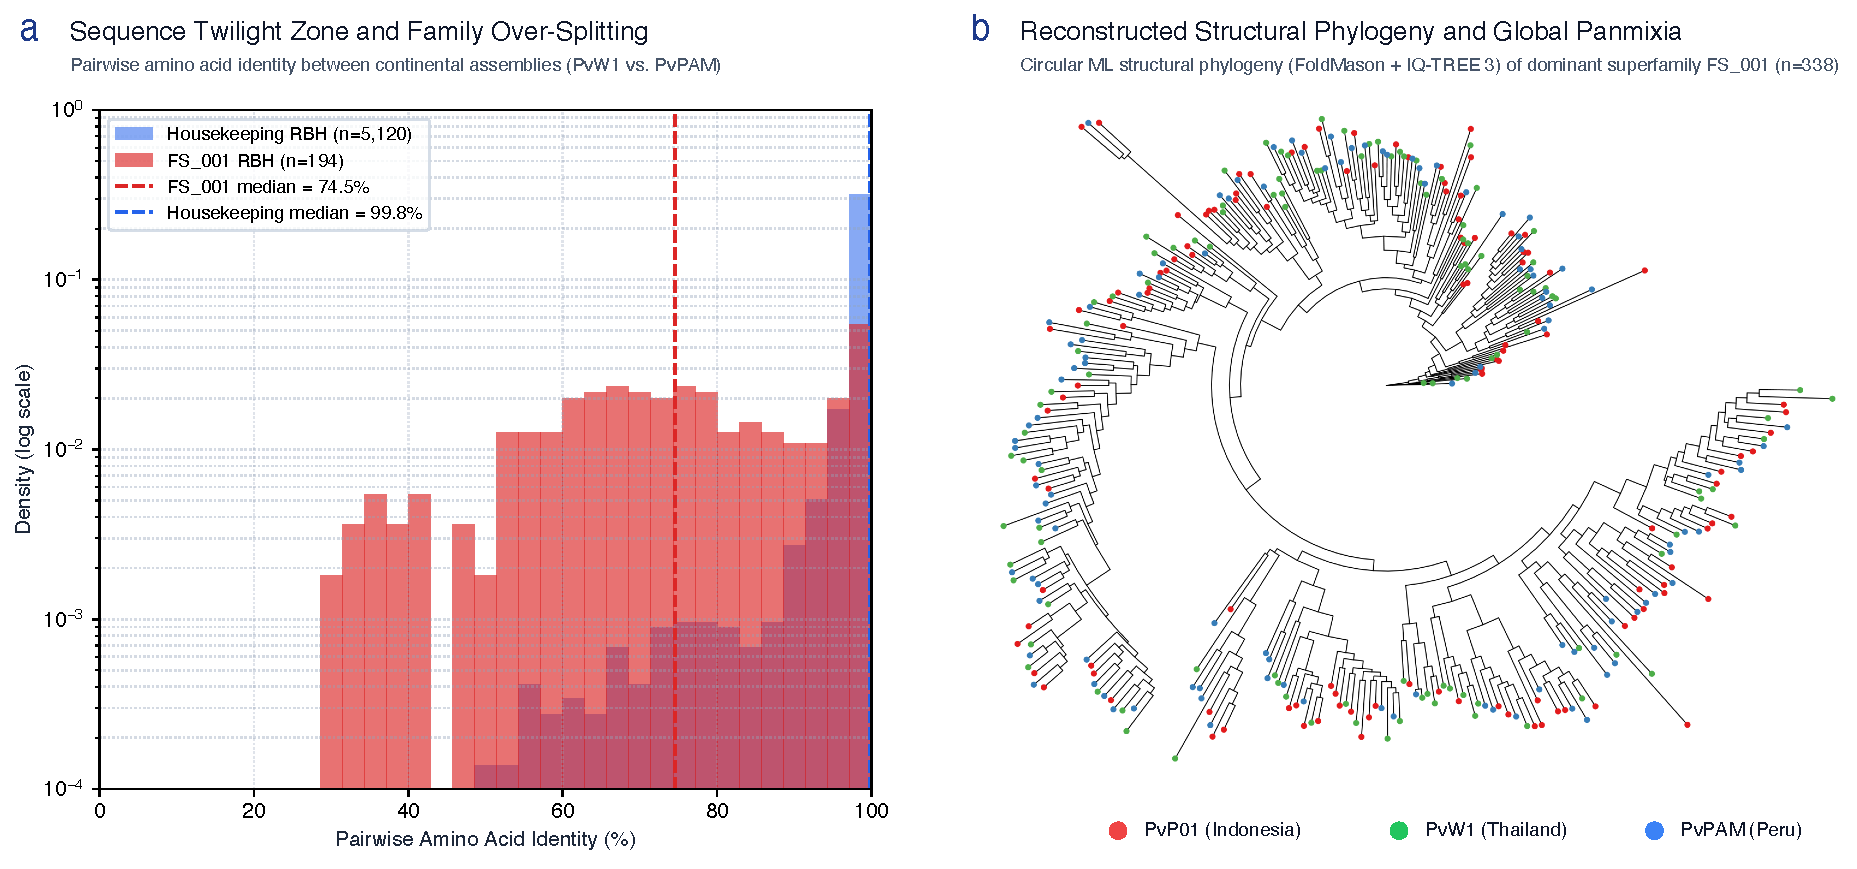
\includegraphics[width=0.92\textwidth]{figures/figure3_vir_reconstruction.pdf}
\caption{\textbf{Structure-aware family reconstruction and ancestral lineage sharing of \textit{Plasmodium vivax} VIR surface antigens across continental genomes.} 
\textbf{A}, Sequence twilight zone and structural unification of over-split subfamilies. Horizontal box-and-strip plots display pairwise amino acid sequence identity between PvW1 (Thailand) and PvPAM (Peru) for conserved single-copy housekeeping genes (median 99.8\%, IQR 0.9\%, amber, $n = 5,120$ pairs) versus VIR pairs within dominant superfamily FS\_001 (median 74.5\%, IQR 25.9\%, Wilcoxon $p = 1.6 \times 10^{-63}$, blue, $n = 194$ pairs). Sequence-only Markov clustering (\texttt{--min-seq-id 0.3}) fractures the 2,592 VIR proteins across Indonesia (PvP01), Thailand (PvW1), and Peru (PvPAM) into 203 sequence clusters (146 subfamilies with $\ge 3$ members). Structure-aware clustering using ProstT5 and Foldseek 3Di representations collapses this repertoire into 73--76 structural classes (24--25 with $\ge 3$ members) across local and UseGalaxy.org execution environments, where the dominant superfamily FS\_001 unifies 89 sequence subfamilies (see Methods). 
\textbf{B}, Circular maximum-likelihood structural phylogeny inferred by IQ-TREE 3 from FoldMason alignments of 338 FS\_001 representatives across Indonesia (PvP01, red, 34.9\%), Thailand (PvW1, blue, 32.5\%), and Peru (PvPAM, green, 32.5\%) using partitioned amino acid and 3Di structural models. Continental lineages are thoroughly interleaved across the tree. A tip-label parsimony permutation test confirms that observed geographic transitions (score $= 160$) match 1,000 random shuffles (null median $160$, $p = 0.55$).}
\label{fig:vir_reconstruction}
\end{figure}

\subsection{Dating emergence of key pathogens across 42 benchmark alignments}

Finally, we tested high-throughput epidemic dating across 42 viral and bacterial benchmark alignments (from 37 publications across 41 outbreaks plus a paired 14.5~kb Ebola coding partition, spanning Ebola, SARS-CoV-2, Zika, Dengue, Chikungunya, Mpox, Influenza, \textit{Mycobacterium abscessus}, and \textit{Yersinia pestis}). Estimating the time to the most recent common ancestor ($t_{\mathrm{MRCA}}$) in BEAST \cite{suchard2018} typically requires hours to days of Bayesian MCMC sampling per alignment. Orbit registered two User-Defined Tools wrapping ChronAeon (\url{https://github.com/veg/chronaeon}) \cite{pond2026hyphaeon} on UseGalaxy.org and dated all 42 alignments concurrently in seconds of manifold computation per dataset inside a single Galaxy history (Figure~\ref{fig:chronaeon_42cohorts}, see Methods).

\begin{figure}[!htbp]
\centering
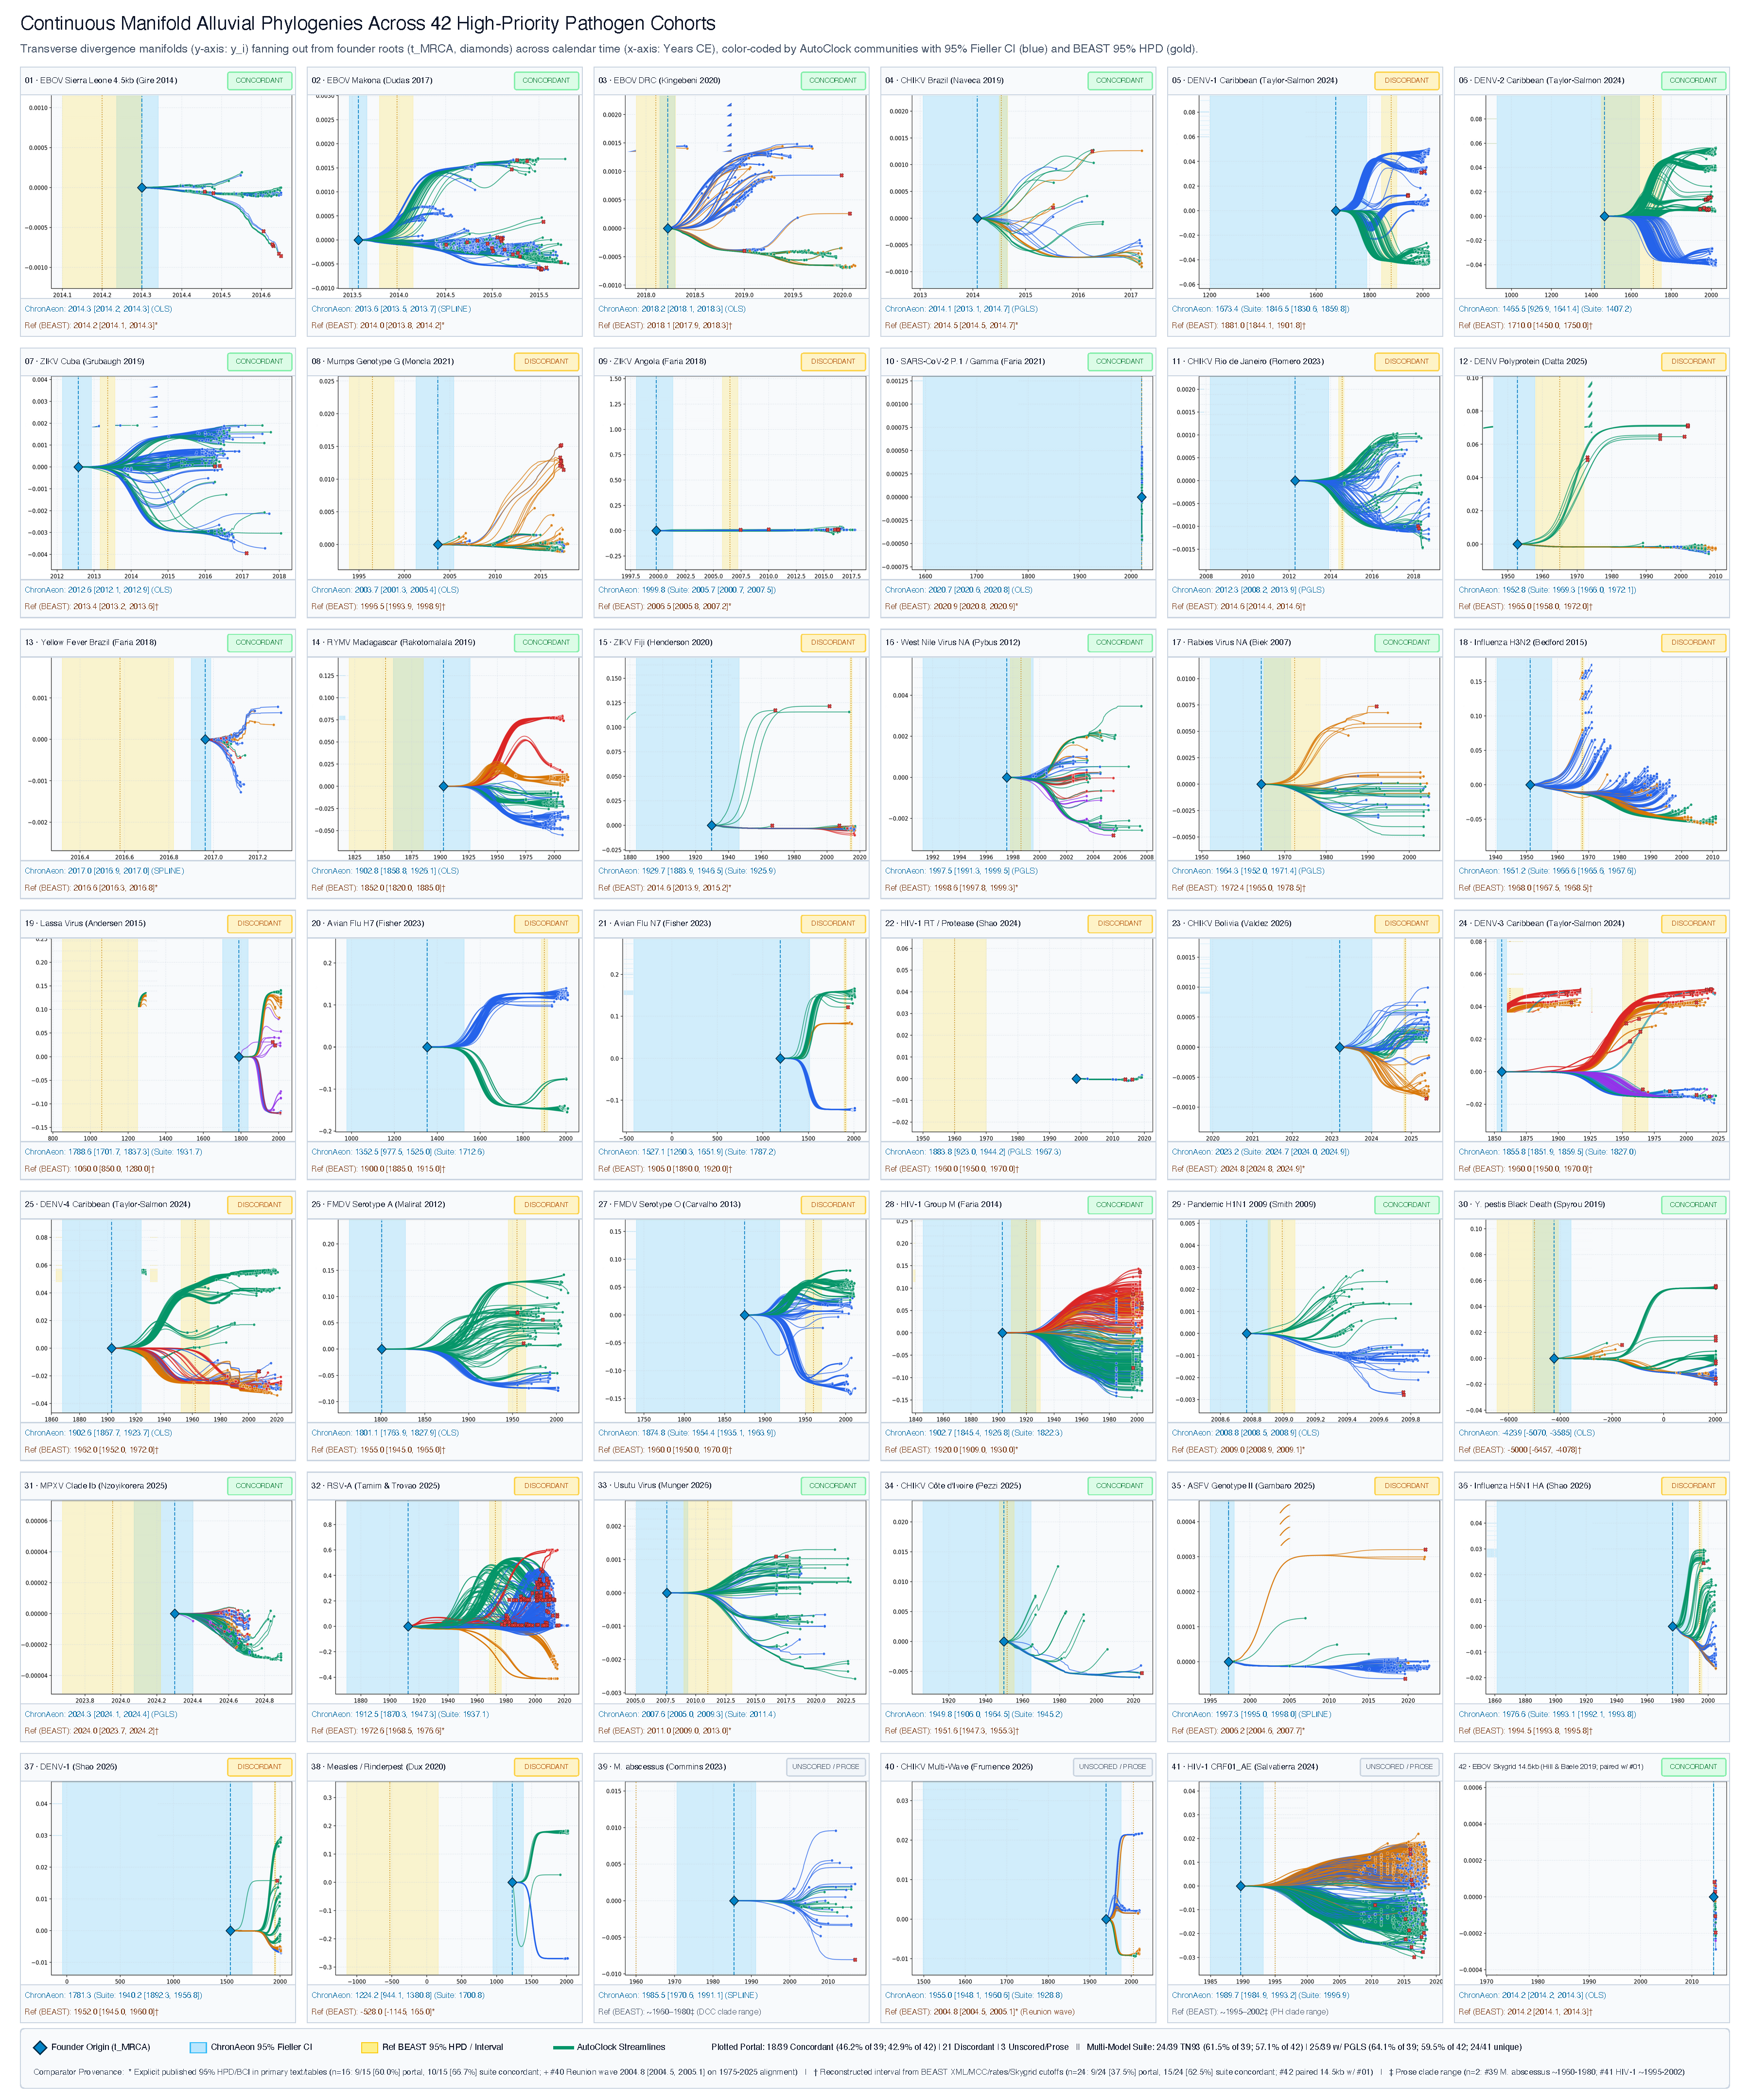
\includegraphics[width=\textwidth,height=0.78\textheight,keepaspectratio]{figures/figure4_chronaeon_42cohorts.pdf}
\caption{\textbf{Continuous manifold alluvial phylogenies and emergence dating across 42 pathogen cohorts on UseGalaxy.org.} 
Each panel displays continuous manifold trajectories fanning out from the inferred epidemic origin ($t_{\mathrm{MRCA}}$, blue diamond) across calendar time, color-coded by AutoClock evolutionary communities ($k \in [0, K^*-1]$) to show lineage expansion and replacement. Shaded bands compare the ChronAeon 95\% Fieller analytical confidence interval (light blue) against the published or reconstructed Bayesian reference interval (gold). Top banners and bottom status strips report the pathogen cohort, primary citation, and concordance of the plotted single-pass baseline against the 39 numeric reference intervals (interval overlap or $|\Delta t_{\mathrm{MRCA}}| < 1.0$~year). Pairwise-distance regression and HyphAeon Attention PGLS match reference Bayesian dates on 25 of 42 alignments (64.1\% of the 39 scored comparators, Supplementary Table~\ref{tab:case3_artifacts}).}
\label{fig:chronaeon_42cohorts}
\end{figure}

Across major recent outbreaks---including 2014 West African Ebola \cite{gire2014genomic, dudas2017virus, hill2019skygrid} and SARS-CoV-2 Gamma \cite{faria2021genomics}, where ChronAeon's estimate ($2020.71$) fell within two months of the published BEAST root ($2020.87$)---tree-free pairwise-distance regression matched reference dates across 61.5\% of the 39 scored cohorts (24 of 39), rising to 64.1\% (25 of 39, median error $0.40$~years across 19 post-1980 outbreaks) with HyphAeon Attention PGLS on Mpox Clade Ib (Supplementary Table~\ref{tab:case3_artifacts}). Preserving every alignment and diagnostic output in a public Galaxy collection also explained the 14 discordant cohorts: unrooted distance regression breaks down on ancient roots compressed by purifying selection and mutational saturation (such as Lassa \cite{andersen2015lassa, suchard2020lassa} and Measles/Rinderpest \cite{dux2020measles}) and on multi-lineage alignments where whole-alignment regression dates a deep species split rather than a regional introduction (see Methods).

\subsection{Putting this all together}

Anyone can use this architecture today (\url{https://galaxyproject.org/agents/}) with a free account and API key on UseGalaxy.org, UseGalaxy.eu, or UseGalaxy.org.au. Command-line users can install \texttt{agentic-plugins} (\url{https://galaxyproject.org/agents/plugins/}) to register \texttt{galaxy-mcp} with curated Galaxy and Workflow Foundry skills, while desktop users can download Orbit for macOS, Linux, or Windows (\url{https://galaxyproject.org/agents/orbit/}) using commercial APIs, ChatGPT subscriptions, or free local Ollama models. Both paths execute every step as a verifiable Galaxy job, and we are embedding a native open-model agent directly inside the Galaxy web interface.

\clearpage
\section{Discussion}

Autonomous agents make complex data analysis feel effortless, allowing any student or investigator to generate polished figures in minutes. As our benchmark and reanalyses show, however, effortless execution routinely masks flawed choices: suppressed reference assemblies that erase expressed toxin genes, eukaryotic spliced aligners applied to bacteria, unpooled dispersion models, or reversed library strandedness. Even more telling is what Orbit uncovered in the recent \textit{Nature} Paper2Agent spatial transcriptomics benchmark \cite{miao2026}. Tasked with reproducing a mouse cortex analysis backed by a 5,613-cell reference atlas \cite{sun2024}, an unguided agent silently substituted a 1,000-cell unit-test file from the repository's \texttt{tests/data/} folder, cutting prediction correlation threefold ($r = 0.0861$ vs.\ $r = 0.2553$). Because the agent ran in an unrecorded local environment and left behind only a static figure, that fivefold loss of reference data went undetected through authorship and peer review. Connecting agents to public Galaxy infrastructure, visual workflow validation, and national supercomputers is designed specifically to prevent such failures by making every dataset, parameter, and analytical shortcut immediately inspectable by authors, collaborators, and reviewers.

Several practical limitations clarify where human expertise and community guardrails remain essential. Whereas our planning benchmark evaluated $n = 10$ independent runs per model family, our live execution comparisons and biological case studies represent interactive sessions that incorporated investigator steering---such as switching HISAT2 to Kallisto in \textit{B.\ cereus}---alongside autonomous forensic audits. Connecting agents to public infrastructure also does not eliminate model-level execution failures, and the record is what makes them diagnosable---failures, including defects in Orbit itself, can be identified after the fact from each session's notebook and activity log rather than from the agent's own summary. Shared infrastructure likewise does not eliminate minor floating-point or thread-scheduling differences across hardware architectures, the ChronAeon clock module was evaluated by its developers (with 24 of 39 reference intervals reconstructed from prose or clock calibrations, see Methods), and commercial model APIs still carry usage costs. In our evaluations, however, skill-guided workflows perform well with open-weight models such as DeepSeek at a fraction of the cost, and serving open models directly on public supercomputers will remove that barrier altogether.

Running agents on public infrastructure also requires balancing extensibility against security and software sprawl. Historically, Galaxy users could only run pre-installed tools, which stalls an agent whenever an analysis needs a custom script or new model. User-Defined Tools (UDTs) solve this by packaging custom scripts or heavy models into isolated containers on demand, but arbitrary container execution on shared clusters requires access controls: UseGalaxy.org grants UDT privileges via an approved account list, whereas UseGalaxy.eu routes requests through an automated packaging and pull-request review pipeline. As binary-decompilation agents such as Reverse Engineer Anything (REA) \cite{rea2026} make software replaceable on demand, thousands of uncurated UDTs could easily degenerate into an unmaintained graveyard no better than thousands of abandoned GitHub repositories, where stars reflect popularity rather than whether code still runs on real data. Shared execution on Galaxy provides a concrete selection and governance mechanism across three stages (see Methods). First, agents register UDTs with mandatory pinned containers and typed schemas in user-scoped histories to unblock immediate analyses without cluttering the global tool panel. Second, platform execution telemetry tracks real-world invocation counts, failure rates, and resource footprints across independent users while flagging duplicate wrappers. Third, recurring high-utility UDTs are routed to the Intergalactic Utilities Commission (IUC) \cite{iuc2026} and Intergalactic Workflow Commission (IWC) \cite{iwc2026}, where human maintainers consolidate redundant wrappers, add Planemo regression tests, and graduate vetted tools into permanent community standards.

Finally, verifiable agentic infrastructure changes what a scientific publication itself represents. When an agent executes a study on public infrastructure, the primary scientific product is no longer a static prose manuscript---it is the immutable Research Object Crate (RO-Crate) of inputs, workflows, container digests, and results archived on Zenodo with a permanent DOI. Once that computational lineage is locked and auditable, multimodal synthesis tools such as NotebookLM can generate written reports, slide decks, or interactive summaries on demand in whatever format a reader prefers, letting scientific communication adapt to any medium without sacrificing rigor.

\section*{Methods}

\subsection*{Multi-Agent Analytical Divergence Benchmark}
We evaluated analytical divergence across autonomous agents using an RNA-seq study of carbohydrate-mediated enterotoxin repression in \textit{Bacillus cereus} (BioProject PRJEB86181, PMC12804731) \cite{vyklicka2026}. The primary contrast compared two glucose-supplemented replicates (ERR14660412 and ERR14660413) against three baseline tryptic soy broth control replicates (ERR14660420, ERR14660421, and ERR14660422) from nineteen RNA-seq libraries across seven growth conditions (six carbohydrate supplements plus tryptic soy broth control, alongside one whole-genome sequencing run, ERR14660405, totaling twenty ENA runs). In the published study, excess glucose represses the primary pore-forming enterotoxin subunit \textit{nheB}, leaves the regulatory subunit \textit{nheC} unchanged, and induces the cell-wall peptidase \textit{entFM}, while diarrheal toxins hemolysin BL (\textit{hbl}) and cytotoxin K (\textit{cytK}) are reported as unexpressed.

To quantify planning variation, we evaluated 30 isolated agents across three foundation model families: ten Claude Opus 5.5 agents (Anthropic Claude Code CLI, \texttt{cc}), ten Codex agents running GPT-6 Astra (OpenAI Codex CLI, \texttt{codex exec}), and ten Gemini 3.8 Flash agents within Antigravity (\texttt{agy}, Google). The version strings designate the frontier Anthropic, OpenAI, and Google CLI model snapshots evaluated in our early-2026 benchmark logs. Each agent received identical natural-language instructions in an empty local workspace directory with no prior session context, external memory, or access to Galaxy cyberinfrastructure (Table~\ref{tab:planning_prompt}). During planning, each agent operated under its native CLI tool permissions: web fetch/search and \texttt{curl} in Claude Code, live web search in a network-restricted shell sandbox in Codex, and URL reading plus shell execution in Antigravity. We parsed each generated plan across eight sequential analytical decisions: reference genome assembly, workflow engine, read trimming software, ribosomal RNA depletion strategy, read aligner, quantified genomic feature, differential expression model scope (19-sample pooled vs.\ 5-sample contrast-only), and log-fold-change shrinkage prior. Combinatorial trajectory diagrams were constructed from this discrete decision matrix. Model families exhibited distinct planning profiles shaped by both model priors and CLI tool permissions. Claude plans aligned to \textit{Bacillus pacificus} anQ-h4 and pooled variance across all nineteen RNA-seq libraries. Codex plans aligned to the sequenced isolate \textit{Bacillus cereus} ATCC 10987 and restricted the comparison to the five target replicates. Gemini plans showed severe instability across assemblies, citing a non-\textit{Bacillus} assembly (\texttt{GCF\_000008105.1}, \textit{Salmonella enterica} serovar Choleraesuis SC-B67) mislabeled as \textit{B.\ cereus} ATCC 10987 in one plan, citing the \textit{B.\ cereus} ATCC 14579 chromosome accession (\texttt{AE016877.1}) for ATCC 10987 in another, and reversing library strandedness in four plans. Aligning against a wrong assembly or genus alters or invalidates gene coordinates and annotations. Inverting library strandedness discards or miscounts real transcripts. Pooling all nineteen libraries to estimate variance alters statistical power compared to analyzing only the five target replicates.

\begin{table}[!htbp]
\centering
\footnotesize
\begin{tabularx}{\textwidth}{X}
\toprule
\textbf{Standardized Planning Prompt Dispatched to All Thirty Agents} \\
\midrule
You are a bioinformatics expert. Task: \par\vspace{0.4em}
Paper: Bacillus cereus RNA-seq study, PMC12804731 (\url{https://www.ncbi.nlm.nih.gov/pmc/articles/PMC12804731/}). Read the paper (and its data availability / methods sections, and any linked GEO/SRA/BioProject accessions) yourself using web access. \par\vspace{0.4em}
Goal: Replicate the primary comparison --- Glucose vs. TSB control --- 5 samples total: 2 treatment (glucose) and 3 control (TSB). \par
Constraint: Do NOT use Galaxy (no Galaxy servers, Galaxy tools/workflows, Galaxy skills or infrastructure). \par\vspace{0.4em}
DO NOT perform the analysis, do not download data, do not install software. Produce ONLY a detailed analysis PLAN. \par\vspace{0.4em}
The plan must be detailed and concrete, covering at minimum: \par
1. Summary of the paper's design and what it reports for this comparison (and what you could/could not verify from the paper). \par
2. Data acquisition: exact accessions (BioProject/GEO/SRA run IDs if findable), how to fetch (tools/commands). \par
3. Reference genome and annotation: exact strain/assembly accession (RefSeq/GenBank), annotation source/format, plasmids, rationale, alternatives considered. \par
4. Compute environment: language, package/environment manager, workflow manager (if any), containers, hardware estimates. \par
5. Step-by-step pipeline with specific tools AND versions and key parameters: QC, trimming, rRNA handling, alignment or pseudo-alignment, quantification, strandedness detection, counting rules (multi-mappers, overlaps, feature type e.g. CDS/gene/locus\_tag), post-alignment QC, MultiQC. \par
6. Differential expression: tool(s), normalization, design formula, handling of n=2 vs n=3 (low replication), dispersion/shrinkage, thresholds (padj, log2FC), multiple testing. \par
7. Downstream/functional analyses: annotation (GO/KEGG/COG, eggNOG etc.), enrichment method, operon/regulon considerations, specific pathways expected for glucose (e.g. CcpA catabolite repression, glycolysis, toxins), visualization (PCA, volcano, MA, heatmaps). \par
8. Validation / replication criteria: how you will compare your results to the paper's reported results (concordance metrics, gene lists, figure reproductions). \par
9. Key decision points and alternatives (where reasonable analysts would differ), risks and pitfalls. \par
10. Reproducibility deliverables (repo layout, scripts, lockfiles, reports). \par\vspace{0.4em}
IMPORTANT: This is a NON-INTERACTIVE run. Nobody can answer questions --- never ask the user anything or offer options, make reasonable decisions yourself and state assumptions. If a page cannot be fetched, try alternatives (e.g. Europe PMC REST API \url{https://www.ebi.ac.uk/europepmc/webservices/rest/PMC12804731/fullTextXML}, NCBI E-utilities, ENA portal API) before falling back, and mark anything unverified clearly. \par\vspace{0.4em}
Output the complete plan as Markdown in your final answer (nothing else). Work independently, and do not read or write any local files other than what you need to think --- the final plan must be in your answer text. \\
\bottomrule
\end{tabularx}
\caption{\textbf{Standardized natural-language prompt dispatched to thirty autonomous agents.} All agents received this identical prompt in an isolated workspace with no inter-session memory or access to Galaxy cyberinfrastructure. The prompt directed agents to formulate an end-to-end analysis plan across ten explicit criteria without human intervention or external workflow platforms.}
\label{tab:planning_prompt}
\end{table}

For empirical re-analysis, three agents executed end-to-end replications on dedicated host hardware. Runs used Gemini 3.8 Flash (Antigravity CLI), Claude Opus 5.5 (Claude Code), and Codex (GPT-6 Astra) on an Ubuntu Linux workstation (24 CPU cores, 62~GB RAM, NVMe storage). During live execution, each agent was instructed to fetch the five target RNA-seq libraries from the European Nucleotide Archive, perform quality control, align reads, quantify gene-level abundances, and estimate differential expression for target enterotoxin genes (\textit{nheA}, \textit{nheB}, \textit{nheC}, \textit{entFM}, \textit{cytK}, and the \textit{hbl} operon), with freedom to select its alignment and modeling stack. Gemini executed an ad-hoc bash script driving Bowtie2 v2.5.5 and unstranded featureCounts v2.1.1 on \textit{Bacillus pacificus} anQ-h4 (unshrunken Wald $\log_2\text{FC} = -2.41$, $p_{\text{adj}} = 0.0021$ for \textit{nheB}, and $\log_2\text{FC} = +1.42$, $p_{\text{adj}} = 0.0658$ for \textit{entFM}, with \textit{nheC} $p_{\text{adj}} = \texttt{NA}$ after independent filtering, raw $p = 0.51$). Whereas all ten Claude planning runs proposed pooling all nineteen libraries on \textit{B.\ pacificus} anQ-h4, during live execution Claude Code analyzed the five target samples and aligned reads against the sequenced isolate \textit{Bacillus cereus} ATCC 10987 (\texttt{GCF\_000008005.1} / \texttt{GCA\_000008005.1}, NCBI BioProject \texttt{PRJNA74}, where RefSeq later suppressed \texttt{GCF\_000008005.1} over frameshifted CDS annotations). The Claude Code run used containerized nf-core/rnaseq 3.14.0 and nf-core/differentialabundance 1.4.0 under Docker, consuming over 100~GB of scratch disk. Aligning to ATCC 10987 recovered active baseline transcription of the cytotoxin K locus (\texttt{BCE\_1209} / \texttt{BCE\_RS06135}, 548--1,420 raw read pairs per library, mean 797, DESeq2 $\text{baseMean} = 831$, non-differentially expressed, $\log_2\text{FC} = +0.58$, $p_{\text{adj}} = 0.43$), which was reported as undetected in the published study, consistent with alignment against \textit{B.\ pacificus} anQ-h4 (an assembly lacking \textit{cytK}). Claude Code's nf-core/differentialabundance pipeline output \texttt{ashr}-shrunken posterior effect sizes and standard deviations, replicating \textit{nheB} repression ($\log_2\text{FC} = -2.08$, $p_{\text{adj}} = 0.0002$) and \textit{entFM} directional induction ($\log_2\text{FC} = +1.08$, $p_{\text{adj}} = 0.0620$). Codex replaced its planned Snakemake pipeline with fourteen custom Bash, Python, and R scripts executing HISAT2 and unshrunken DESeq2 Wald tests with dual-reference sensitivity checks across both anQ-h4 and ATCC 10987 (replicating \textit{nheB} $\log_2\text{FC} = -2.16$ to $-2.46$, $p_{\text{adj}} < 10^{-4}$, and \textit{entFM} $\log_2\text{FC} = +1.32$ to $+1.35$, $p_{\text{adj}} \le 0.0220$, with anQ-h4 \textit{nheC} $p_{\text{adj}} = \texttt{NA}$, raw $p = 0.66$). We captured all generated shell scripts, Conda environments, Docker layer footprints, and execution logs to measure toolchain overlap, disk consumption, and provenance persistence (Supplementary Tables~\ref{tab:agent_resources} and~\ref{tab:agent_scripts}).

\subsection*{Galaxy-Native Replication of \textit{Bacillus cereus} RNA-seq}
To evaluate interactive agent-assisted replication on public cyberinfrastructure, we connected the Antigravity CLI (\texttt{agy}) to UseGalaxy.org through the Galaxy MCP server (\texttt{galaxy-mcp}) \cite{galaxymcp2026}. The five target RNA-seq libraries from BioProject PRJEB86181---two glucose-supplemented replicates (ERR14660412 and ERR14660413) and three tryptic soy broth control replicates (ERR14660420, ERR14660421, and ERR14660422)---were imported into a Galaxy history. We also staged the \textit{Bacillus cereus} ATCC 10987 reference genome (\texttt{GCF\_000008005.1} / \texttt{GCA\_000008005.1}, BioProject \texttt{PRJNA74}) and RefSeq coding sequence transcriptome (4.59~Mb across 5,476 FASTA records mapping to 5,472 unique coding loci, Supplementary Table~\ref{tab:brc_artifacts}).

Before launching the full analysis, the agent validated its workflow on a 1,000-read pilot subset. In NCBI RefSeq bacterial CDS FASTA exports, genes containing programmed ribosomal frameshifts or internal stop codons are split across multiple coordinate intervals that share the same locus tag with numerical suffixes (\texttt{\#1}, \texttt{\#2}). Because Kallisto index construction rejects duplicate target identifiers, the agent deduplicated these split headers on the pilot subset before processing the full libraries.

After we directed the agent to replace its initial eukaryotic spliced aligner (HISAT2) with prokaryotic Kallisto pseudoalignment---because spliced alignment on an intronless bacterial genome searches for nonexistent introns, risks spurious split-read mappings across repetitive toxin loci, and writes multi-gigabyte intermediate BAM files---the agent assembled and validated a reusable Galaxy workflow combining FastQC, fastp, Kallisto quant \cite{bray2016near}, DESeq2, and MultiQC (Supplementary Table~\ref{tab:brc_artifacts}). During workflow construction, Galaxy's workflow schema validator enforces strict input-output type compatibility across connected steps. When the agent initially wired a standalone \texttt{tximport} step between Kallisto's output collection of transcript-level abundance tables and DESeq2's collection-mode input, the editor flagged the single-table-to-collection mismatch in orange (Figure~\ref{fig:bacillus_replication}A). Inspecting the validation response returned by the MCP server, the agent removed the standalone \texttt{tximport} step, generated a two-column transcript-to-gene mapping table (\texttt{tx2gene.tsv}), and configured DESeq2's integrated \texttt{tximport} mode to aggregate collection-level transcript abundances into gene-level counts (Figure~\ref{fig:bacillus_replication}B). Under glucose supplementation in this five-library single-contrast design ($n = 2$ glucose vs.\ $n = 3$ control replicates), primary lytic enterotoxin subunit \textit{nheB} decreased 5.05-fold ($\log_2\text{FC} = -2.335$, $p_{\text{adj}} = 2.99 \times 10^{-3}$). Subunit \textit{nheA} decreased 2.80-fold ($\log_2\text{FC} = -1.484$, raw $p = 0.0274$, $p_{\text{adj}} = 0.106$, HISAT2 $p_{\text{adj}} = 0.0917$), cell-wall enterotoxin \textit{entFM} was induced 2.70-fold ($\log_2\text{FC} = +1.432$, raw $p = 0.0158$, $p_{\text{adj}} = 0.0730$, HISAT2 $p_{\text{adj}} = 0.0785$), and regulatory subunit \textit{nheC} remained unaffected ($\log_2\text{FC} = -0.158$, raw $p = 0.843$, $p_{\text{adj}} = 0.907$). Both \textit{nheA} and \textit{entFM} reached nominal significance (raw $p < 0.05$) while falling just above the 5\% false discovery rate threshold after Benjamini--Hochberg adjustment across the 2,815 loci passing DESeq2 independent filtering. To verify that unspliced pseudoalignment against coding sequences matched whole-genome spliced alignment, we also ran a parallel HISAT2 and featureCounts pipeline against the full 5.43~Mb genome assembly. On UseGalaxy.org, Kallisto pseudoalignment completed in 38--60~seconds per library without generating intermediate BAM files, compared with 3--5~minutes per library for HISAT2 alignment and coordinate sorting on standard Galaxy workers ($\sim 5\times$ faster, and 4.0--4.8~hours when HISAT2 jobs encountered worker contention, Supplementary Table~\ref{tab:brc_artifacts}). Across the 5,250 expressed bacterial coding loci with non-missing fold-change estimates (of 5,472 total coding loci), Kallisto pseudoalignment and HISAT2 spliced alignment produced near-identical $\log_2$ fold-change estimates (Pearson $r = 0.9622$, $R^2 = 0.9257$). Auditing the interactive Galaxy Page notebook against the replication history confirmed that all embedded dataset references and fold-change tables resolve to verified history outputs (Supplementary Table~\ref{tab:brc_artifacts}).

\subsection*{Galaxy MCP Server and Modular Skills}
Agents interact with computational infrastructure through the Galaxy MCP server (\texttt{galaxy-mcp}) \cite{galaxymcp2026}, which implements an open standard for tool execution and data inspection. Instead of composing shell commands or ad-hoc API scripts for Galaxy work, agents call the server's structured operations (45 in \texttt{galaxy-mcp} v1.11.2). These endpoints enable agents to search tool registries, inspect dataset collections, launch workflows, and monitor execution states through standard input-output streams or remote HTTP connections. The reference server is implemented in Python using the BioBlend library to communicate with the Galaxy REST API. A TypeScript implementation of the same operation set (\texttt{@galaxyproject/galaxy-ops}) is held to a shared contract with the Python server, and Orbit v0.8.0 exposes the Python server to its agent. Transport mechanisms include standard input-output (stdio) for local CLI integration and streamable HTTP for web and remote clients. Authentication occurs through long-lived Galaxy API keys or OAuth2 token exchanges supplied via environment variables (\texttt{GALAXY\_API\_KEY}). The server provides structured error handling and schema validation across all parameter endpoints.

Domain expertise is provided through modular skill packages \cite{galaxyskills2026} that teach language models standard bioinformatics conventions. Skills guide tool discovery, parameter selection, and collection manipulation idioms. For complex multi-step pipelines, Workflow Foundry skills compile validated workflow templates into agent memory \cite{foundry2026}. By separating operational skills from the underlying compute runtime, the framework steers agents toward community-vetted analytical procedures rather than improvised ones. Skills are guidance, not enforcement---an agent can still deviate from them, which is why the execution record matters.

\subsection*{User-Defined Tool Architecture}
User-Defined Tools are written in YAML adhering to the \texttt{GalaxyUserTool} class definition. The tool wrapper specifies a mandatory container image hosted on public registries (Quay.io, Docker Hub), typed input parameters, declared output datasets, and an execution command. Commands are templated using sandboxed ECMAScript evaluation executed inside an isolated V8 runtime. Output files are claimed from the working directory through \texttt{from\_work\_dir} designations or dynamic dataset discovery patterns. On public servers, UDT execution is governed by instance-specific access controls (approved account access lists on UseGalaxy.org and automated pull-request packaging queues on UseGalaxy.eu) and platform execution telemetry that tracks invocation counts, failure rates, and resource usage to route recurring wrappers to the Intergalactic Utilities Commission (IUC) \cite{iuc2026} and Intergalactic Workflow Commission (IWC) \cite{iwc2026} for Planemo regression testing.

\subsection*{Orbit Workbench and Execution Guard}
Orbit is an Electron desktop application around a headless agent runtime built as an extension on Pi.dev, and the same runtime also runs as a terminal client. The description below reflects Orbit v0.8.0. The analysis directory is the unit of work. Plans, decisions, and results are Markdown sections of a single \texttt{notebook.md}, which Orbit versions automatically in Git repositories it manages. When the agent submits a Galaxy workflow or tool run, it records the run in the notebook as a YAML block (\texttt{loom-invocation}, \texttt{loom-job}). From then on, a background poller checks Galaxy every 15 seconds without invoking the model, writes the run's status back into the block (text the model can still edit in this release), and flags a workflow that has failing jobs while others are still running. Galaxy finishing a run is kept separate from the result being checked. When a run completes or fails, Orbit prompts the agent to verify the outputs or investigate the failure so the researcher does not have to relay the notification (sending at most three consecutive follow-ups by default, with user input or Stop taking precedence). The notebook can be bound to a Galaxy Page on the analysis history and pushed to it, storing the narrative record alongside the datasets it describes.

Orbit enforces some rules in code and advises others under its default permission settings. An execution guard intercepts \texttt{bash}, \texttt{read}, \texttt{write}, and \texttt{edit} calls through Pi.dev lifecycle hooks and returns allow, ask, or deny from classifiers for shell hazard, sensitive-file reads, path containment, and model tier, where models classified as weaker by name and price receive stricter treatment of sensitive and out-of-workspace file access. Writes outside the workspace and its configured roots require approval, reads of recognized credential stores are denied, and the API keys Orbit holds are redacted by value from tool results and from the result summaries in the session activity log (\texttt{activity.jsonl}). Recognized destructive Galaxy operations require user confirmation and are denied when no user is present to give it. Duplicate or fanned-out SRA imports through the standard download tools are refused before they reach Galaxy, and \texttt{/execute} and \texttt{/run} refuse to start without a readable notebook or, for a plan with pending remote steps, a Galaxy connection. An optional operating-system sandbox confines shell writes beneath the guard. Skills are advisory, as are two checks on the plan: when a plan is drafted without consulting the IWC workflow registry, Orbit sends one follow-up asking the agent to check, and in v0.8.0 it logs, without blocking, a plan step marked complete while the workflow invocation bound to it is still in progress. In our harness evaluations on open-weight models served through TACC (\texttt{evals/} in the Orbit repository), a prompt-only rule requiring approval before writing a plan to the notebook was followed in 0 of 15 graded runs (Qwen3 collapsed the four-stage protocol to two stages, and Llama~3.3 wrote to the notebook on its first turn). In response, the development version following v0.8.0 refuses by default to let a plan step be marked complete while its bound Galaxy run is still in progress---a default adopted after twelve scripted sessions, each run in triplicate, showed that every refusal was a true positive and that honest completions recorded in notebook blocks were let through (\texttt{docs/evidence-gate-audit.md}).

\subsection*{Workflow Foundry and BRC-Analytics}
Galaxy Workflow Foundry (\texttt{@galaxy-foundry/gxwf-foundry}) \cite{foundry2026} is a skill-compilation pipeline implemented in TypeScript and Node.js that converts reusable procedural templates (Molds) into agent skills for diverse agent runtimes such as Claude Code, Codex, Antigravity, and Orbit. Each Mold is a Markdown specification carrying Zod-validated YAML frontmatter that declares upstream handoff schemas, design patterns, reference manuals, and downstream output artifacts. Instead of prompting an agent to invent a multi-step workflow in a single pass, Foundry decomposes workflow synthesis into staged skills that pass structured JSON and Markdown handoffs. Staged compilation extracts a structured summary from a published paper, Nextflow pipeline, or CWL workflow, designs the Galaxy interface and collection data-flow topology, resolves curated ToolShed wrappers or User-Defined Tools, and assembles a \texttt{gxformat2} workflow step by step. Synthesized workflows are validated statically using the \texttt{gxwf} validation engine, which verifies graph topology, step connectivity, and tool parameter schemas against official Galaxy XML definitions and Intergalactic Workflow Commission (IWC) exemplars \cite{iwc2026} before automated execution testing via Planemo.

BRC-Analytics (\url{https://brc-analytics.org}) \cite{brcanalytics2026} is the NIAID Bioinformatics Resource Center analytics portal built on public Galaxy infrastructure. It maintains a taxonomy-indexed catalog of curated pathogen, fungal, eukaryotic parasite, and vector reference assemblies, gene annotations, and public sequencing runs aggregated from NCBI Assembly, RefSeq, Ensembl, VEuPathDB, and the Sequence Read Archive (SRA/ENA). In autonomous workflows, BRC-Analytics removes the error-prone step of scraping FTP directories, reconciling assembly accession versions across databases, or downloading raw sequencing files to local storage. Agents query BRC-Analytics by taxonomic identifier or BioProject accession to resolve canonical reference FASTA sequences, GTF/GFF3 gene models, and paired or single-end SRA run collections and stage them into a target UseGalaxy.org history with preserved sample metadata.

\subsection*{Spatial Transcriptomics Conformal Uncertainty Reproduction}
To reproduce and scale the spatial transcriptomics benchmark of Miao et al. \cite{miao2026} and Sun et al. \cite{sun2024}, Orbit registered User-Defined Tools \texttt{tissue\_spatial\_prediction} v1.2.0 and \texttt{tissue\_full\_evaluation} v1.0.0 (container \texttt{quay.io/biocontainers/squidpy:1.5.0}, 4 CPU cores) on UseGalaxy.org (Supplementary Table~\ref{tab:case1_artifacts}). The tools implement SpaGE principal-vector domain adaptation (10 principal vectors) and fixed-radius $k$-nearest-neighbor spatial graph construction ($k = 15$). They then apply cell-centric variability stratified conformal prediction ($k_g = 4$ gene groups, $k_c = 2$ cell groups, 10-fold cross-validation, random seed 42 for single-gene \textit{Acta2} and 444 for 33-gene evaluation) at nominal coverage $1 - \alpha = 0.77$ ($\alpha = 0.23$) and $0.80$ ($\alpha = 0.20$). Single-gene \textit{Acta2} prediction and 10-fold spatial cross-validation workflows across all 33 osmFISH panel genes were executed on UseGalaxy.org across two reference datasets. The two reference cohorts comprised the 1,000-cell tutorial subset (\texttt{tests/data}: \texttt{Spatial\_count.txt}, \texttt{Locations.txt}, and \texttt{scRNA\_count.txt}, 1,000 reference cells $\times$ 33 osmFISH panel genes) and the complete Zenodo Dataset 15 archive (3,405 somatosensory cortex osmFISH spatial cells $\times$ 33 genes paired with 5,613 scRNA-seq reference cells $\times$ 30,527 genes, subsetted to the 33 shared panel genes). On the 1,000-cell tutorial subset (31 calibration genes after TISSUE's default 1\% \textit{Flt1} filter, or 32 unfiltered), local and Galaxy UDT runs matched predicted expression to floating-point precision ($r = 1.0000$, $\Delta_{\max} < 10^{-15}$). Stochastic $k$-means stratification yielded empirical coverage of 86.46\% on Galaxy (86.49\% locally) at $\alpha = 0.23$, mean $\log(1 + \text{PI Width})$ of 2.0621 (2.0634 locally), and colorbar range $[1.89, 2.35]$ (95th percentile 2.3552). By comparison, Extended Data Figure 1c of Miao et al.\ reported a $[2.00, 2.32]$ colorbar on the 1,000-cell tutorial subset, where $k$-means stratification shifts high-uncertainty cells between the ventral boundary and pial edge. On the full 5,613-cell Dataset 15 reference, single-gene \textit{Acta2} prediction (seed 42, 32 unfiltered calibration genes) raised correlation from $r = 0.0861$ to $r = 0.2553$ at 85.61\% coverage. In the 33-gene 10-fold cross-validation workflow (seed 444, 31 calibration genes after TISSUE's default 1\% \textit{Flt1} filter), \textit{Acta2} reached $r = 0.2845$ and 81.03\% coverage, while overall 33-gene coverage reached 79.05\% at nominal 77\% and 81.33\% at nominal 80\% (Supplementary Table~\ref{tab:case1_artifacts}).

\subsection*{Pathogen and Vector Genomics Reanalyses on UseGalaxy.org}
For the 30-sample \textit{Aspergillus fumigatus} itraconazole time-course of Hokken et al. \cite{hokken2018} (BioProject PRJNA482512, three clinical isolates sampled at 0, 30, 60, 120, and 240 minutes in duplicate), BRC-Analytics staged the Af293 reference genome (Ensembl Fungi ASM265v1) and 30 paired-end SRA runs into a UseGalaxy.org history (Supplementary Table~\ref{tab:brc_artifacts}). Workflow Foundry compiled a 60-step workflow chaining \texttt{fastp}, \texttt{rna\_star} (\texttt{--quantMode GeneCounts}), unstranded count extraction (verified by forward-to-reverse STAR strand column ratios of 0.979--1.007 across ten libraries), and pooled 30-sample one-factor five-level timepoint \texttt{deseq2} (\texttt{\textasciitilde timepoint}). Under the published study's three simultaneous significance thresholds ($\text{baseMean} \ge 30$, $p_{\text{adj}} < 0.1$, and $|\log_2\text{FC}| > 1$), four separate 12-sample pairwise fits inflated standard errors by 18--26\% and missed 31\% of differentially expressed genes (DEGs) at 120 minutes and 39\% at 240 minutes, recovering only 82 of 186 consistent DEGs. By contrast, the pooled 30-sample model reproduced published standard errors to four decimal places ($\log_2\text{FC}$ Pearson $r = 0.9996\text{--}0.9999$). It identified 3,922 vs.\ 3,955 DEGs at 30 minutes, 3,393 vs.\ 3,430 at 60 minutes, 1,191 vs.\ 1,207 at 120 minutes, and 1,098 vs.\ 1,101 at 240 minutes, recovering 185 consistently differentially expressed genes against the published 186 (181 shared). Three custom User-Defined Tools (\texttt{hokken\_go\_enrichment}, \texttt{hokken\_venn\_comparison}, and \texttt{hokken\_revigo\_summary}) replaced the decommissioned AspGD GO Term Finder and interactive REVIGO browser utility while automating cross-namespace \texttt{AFUA\_}/\texttt{Afu} Venn overlap comparisons (benchmarked against BioVenn). Together, the three UDTs reproduced both the temporal enrichment inversion (135 upregulated vs.\ 2 downregulated terms at 30 minutes, reversing to 0 upregulated vs.\ 136 downregulated terms at 240 minutes) and the expression trajectories of the 61-gene drug-efflux transporter panel (\textit{mdr1}, \textit{mdr4}, \textit{abcA}, \textit{abcC}, and \textit{mfs56}).

For the \textit{Anopheles gambiae} infection chromatin study of Ruiz et al. \cite{ruiz2021} (GEO GSE152924, \texttt{SRR12064732}--\texttt{SRR12064735}), reads were aligned to AgamP4 with Bowtie2, filtered for $\text{MAPQ} \ge 10$, and deduplicated. Sub-nucleosomal fragments ($< 130$~bp) were shifted by $+4/-5$~bp via UDT \texttt{ruiz\_tn5\_fragment\_extractor} and called with historical MACS2 2.1.2 via UDT \texttt{ruiz\_macs2\_212\_narrowpeak} (\texttt{-f BAMPE -g 273109044 -q 0.01 -B --keep-dup all --nomodel --nolambda}, alongside single-end shifted \texttt{--shift -100 --extsize 200} sensitivity checks on the Galaxy MACS2 2.1.1 wrapper, Supplementary Table~\ref{tab:brc_artifacts}). Measured at the stated 51\% reciprocal-overlap criterion against the authors' deposited regions, independent MACS2 2.1.2 calls recovered 92.4\% and 93.2\% of reported midgut regions and 90.7\% and 93.2\% of reported salivary-gland regions. Counting merged consensus intervals on strict 50--130~bp MACS2 2.1.1 peaks yielded only 9,448 midgut and 19,502 salivary-gland intervals against the published 43,010 and 68,576 (or 21,841 and 31,513 under relaxed calling and 21,775 and 30,844 without deduplication). By contrast, applying the 51\% reciprocal-overlap rule row-wise per replicate to unmerged $< 130$~bp peaks recovered 41,580 midgut ($-3.3\%$) and 57,518 salivary-gland ($-16.1\%$) rows on MACS2 2.1.2 (and 41,340 [$-3.9\%$] midgut and 57,274 [$-16.5\%$] salivary-gland rows on the MACS2 2.1.1 wrapper). An empirical near-containment threshold (\texttt{either\_frac} $= 0.851$, where either peak covers at least 85.1\% of the other) reproduced 44,780 midgut ($+4.1\%$) and 67,594 salivary-gland ($-1.4\%$) rows along with assigned genes, promoters, and candidate enhancers within 0.4--4.6\%. A pre-registered cross-tissue transfer test (\texttt{ruiz\_either\_frac\_crossfit}) returned an explicit \texttt{TRANSFER INCONCLUSIVE} verdict (transfer error 7.16\% vs.\ 5.0\% pre-registered threshold) because midguts and salivary glands exhibited distinct single-tissue optima (\texttt{0.884} vs.\ \texttt{0.821}).

For the \textit{Aedes aegypti} midgut single-cell atlas of Wang et al. \cite{wang2024} (\texttt{SRR26591148} and \texttt{SRR26591149}), 10x Genomics 3' v3 reads were aligned to AaegL5.0 (\texttt{GCF\_002204515.2}) with \texttt{rna\_starsolo} and filtered with \texttt{dropletutils} (\texttt{emptyDrops lower=500}). Singlets were quality-controlled in Scanpy after prefixing VectorBase mitochondrial loci with \texttt{MT\_} ($100\text{--}2,500$ genes/cell and $< 20\%$ mitochondrial reads, compared with the published Seurat workflow using $< 30\%$ mitochondrial reads without \texttt{emptyDrops}), retaining 6,707 post-QC cells (3,836 in \texttt{SRR26591148} at Louvain resolution 0.25 and 2,871 in \texttt{SRR26591149} at resolution 0.75 vs.\ 7,147 published). Cells were harmonized into three conserved coarse populations across 5,953 cells (\texttt{EC/digestive broad}: 3,331 and 2,004 cells, \texttt{HC-like/epithelial}: 73 and 213 cells, and \texttt{VM-like}: 257 and 75 cells, with 754 cells in minor replicate-specific clusters). Sample-blocked pseudobulk \texttt{edgeR} (\texttt{\textasciitilde 0 + coarse\_label + sample\_id} across $n = 2$ biological replicates, 6 pseudobulk profiles) across 8,248 expressed genes identified 1,784, 943, and 854 differentially expressed genes ($\text{FDR} \le 0.05$) across the pairwise contrasts. Pseudobulk testing recovered Table S1 markers including enterocyte marker \texttt{AAEL027580} (rank 1 in enterocyte vs.\ hemocyte-like, $\text{FDR} = 2.2 \times 10^{-6}$), visceral muscle markers \texttt{AAEL024504} (rank 1 in enterocyte vs.\ visceral muscle), \texttt{AAEL012704} (rank 1 in hemocyte-like vs.\ visceral muscle and rank 21 in enterocyte vs.\ visceral muscle), and muscle actin \texttt{AAEL001673} (rank 250, $\text{FDR} = 0.002$). It also recovered canonical digestive enzymes including zinc carboxypeptidase (\texttt{AAEL001863}, rank 309) and female-specific chymotrypsin (\texttt{AAEL003060}, rank 531, $\text{FDR} < 0.001$, Supplementary Table~\ref{tab:brc_artifacts}).

\subsection*{Structure-Aware Phylogenomics of \textit{Plasmodium vivax} VIR Antigens}
Annotated proteomes, GFF3 gene models, and genome assemblies for \textit{Plasmodium vivax} isolates PvP01 (Indonesia, short-read Illumina assembly with improved subtelomere scaffolding \cite{auburn2016}), PvW1 (Thailand, long-read assembly \cite{minassian2021pvw1}), and PvPAM (Peru, long-read assembly \cite{demeulenaere2023}) were screened against Pfam profile PF05795 using HMMER 3.4 (\texttt{hmmer\_hmmsearch/3.4+galaxy0}) alongside six-frame pseudogene rescue via UDT \texttt{anton-1-gff\_pseudogene\_translator}. Domain screening identified 2,664 PF05795-positive VIR proteins (931 PvP01, 748 PvW1, and 985 PvPAM), of which 2,592 functional VIR proteins (897 PvP01, 735 PvW1, and 960 PvPAM) passed length filtering into structure-aware clustering. Sequence-only baseline clustering used MMseqs2 v18.8cc5c (\texttt{-e 1e-5 --min-seq-id 0.3 -c 0.5}) and MCL v22.282 ($I = 2.0$), producing 203 sequence clusters (146 subfamilies with $\ge 3$ members). Structure-aware 3Di embedding and clustering used Foldseek v10.941cd33 with ProstT5 weights (\texttt{-c 0.8 -e 0.001 --alignment-type 2}), producing 73 structural classes (24 with $\ge 3$ members, dominant superfamily FS\_001 $= 1,197$ proteins, 46.2\% of the repertoire, merging 89 sequence subfamilies) on the verified local CPU reference branch. On UseGalaxy.org, the same tool produced 76 structural classes (25 with $\ge 3$ members) on an ACCESS-CI NVIDIA A100 GPU via UDT \texttt{anton-gpu-xl-foldseek\_prostt5\_clustering} (FS\_001 $= 812$ proteins, 336 sub-cluster representatives) and on a 32-core Galaxy CPU node via UDT \texttt{anton-32-foldseek\_prostt5\_clustering} (FS\_001 $= 766$ proteins). We did not isolate the exact container or thread-scheduling step responsible for the 73-cluster (local CPU) versus 76-cluster (Galaxy GPU and CPU) split. Across all branches, 21 structural classes contained members from all three continental genomes and held 97.3\% (local CPU) to 97.6\% (Galaxy GPU) of all VIR proteins, whereas 47 single-genome classes accounted for 2.0\% of the repertoire (Supplementary Table~\ref{tab:case2_artifacts}). Lockstep amino acid and 3Di multiple sequence alignment of FS\_001 sub-cluster representatives ($n = 338$ local: 118 Indonesia [34.9\%], 110 Thailand [32.5\%], and 110 Peru [32.5\%], and $n = 336$ GPU branch, subsampled via MMseqs2 \texttt{--min-seq-id 0.5 -c 0.8 --cov-mode 0}) was performed with FoldMason v4.dd3c235 inside custom container \nolinkurl{quay.io/nekrut/foldmason-prostt5:4.dd3c235-cpu} (UDT \texttt{anton-32-foldmason\_align}). Column-occupancy trimming (\texttt{trimAl -gt 0.65}) on the Galaxy branch retained 176 of 336 representatives whereas the verified local CPU reference branch retained all 338 representatives. Partitioned maximum-likelihood phylogenetic inference in IQ-TREE 3 (amino acid VT+F+R6 and 3Di Garg-Hochberg models, 1,000 ultrafast bootstrap replicates) and 1,000-shuffle Fitch parsimony permutation testing (observed score $= 160$ vs.\ null median $160$, mean $159.2 \pm 3.8$, range $145\text{--}177$, $p = 0.55$) are therefore reported from the 338-tip local CPU reference branch. We also mapped chromosomal subtelomere positions (64.5\% within the outer 10\% of chromosomes) and evaluated flanking microsynteny (\texttt{anton-8-mmseqs\_easy\_rbh\_pair} and \texttt{anton-1-microsynteny\_filter}, with 11 of 194 local and 3 of 141 GPU FS\_001 reciprocal best-hit pairs retaining synteny) against 5,120 single-copy housekeeping reciprocal best hits (median identity 99.8\%, 77/77 automated verification checks passed, Supplementary Table~\ref{tab:case2_artifacts}).

\subsection*{Manifold Emergence Dating Across 42 Pathogen Cohorts}
Forty-two curated BEAST XML benchmark alignments (drawn from 37 primary publications across 41 distinct pathogen outbreaks plus a paired 14,517~bp coding tutorial partition, \texttt{41\_skygrid\_rabies\_gill2020}, for the 2014 Sierra Leone Ebola cohort \cite{hill2019skygrid, gill2020skygrid}) were archived on UseGalaxy.org and parsed via UDT \texttt{chronaeon\_batch\_preparator} v1.0.0 into synchronized 42-element BEAST XML, aligned FASTA, and tip-date collections (Supplementary Table~\ref{tab:case3_artifacts}). Concurrent manifold emergence dating was executed across all 42 alignments using UDT \texttt{chronaeon\_cohort\_analysis} v3.2.2 \cite{pond2026hyphaeon}, completing in seconds of core manifold computation per alignment (for example, 2.58~seconds for TN93 AutoClock manifold regression in pilot benchmarking, compared with $5 \times 10^6$ to $10^9$ MCMC states taking 8--36~hours in dual-core BEAST X or 5--7~days in BEAST 2.7.7). During the initial 42-element batch execution on UseGalaxy.org, 5 of 42 container jobs hit a 1-minute \texttt{sed} timeout, were re-executed across recovery runs, and were merged into the final 42-element output collections via \texttt{\_\_BUILD\_LIST\_\_}. For each alignment, the tool computed pairwise evolutionary distances, continuous manifold embeddings, analytical Fieller 95\% confidence intervals \cite{fieller1954some}, leave-one-out cross-validation error, AutoClock normalized Laplacian spectral bisection ($K^*$), and optional HyphAeon Attention PGLS root inference using offline-staged \texttt{model.viral.pt} weights.

To audit reference comparator provenance across all 42 alignments (\texttt{chronaeon\_42cohorts\_provenance.tsv} and Supplementary Table~\ref{tab:chronaeon_comparators}), we classified each cohort's reference interval into three categories. First, 15 alignments had explicit 95\% highest posterior density (HPD) or Bayesian credible intervals (BCI) reported in the primary publication's text or tables (plus \texttt{39\_chikv\_reunion\_dellicour2020} \cite{dellicour2020chikv}, which carries a published BEAST root of $2004.8$ [$2004.5, 2005.1$] in \texttt{published\_comparators.tsv} but was marked \texttt{NO\_COMPARATOR} in the automated runner). Second, 24 alignments had numeric reference intervals in \texttt{aggregate\_benchmark\_results.tsv} reconstructed from prose approximations (such as Hill and Baele's ``approximately March 2014'' TempEst intercept \cite{hill2019skygrid} bracketed as $2014.20$ [$2014.10, 2014.30$], or O'Toole et al.'s late-2015 APOBEC3 emergence estimate \cite{otoole2023mpox}), molecular clock calibrations, or Skygrid grid cutoffs. Third, 2 additional alignments were unscored (\texttt{NO\_COMPARATOR}) in the automated runner and carried prose clade ranges in \texttt{published\_comparators.tsv}: \texttt{38\_mab\_commins2023} (\textit{Mycobacterium abscessus} \cite{commins2023mab}, prose range $\sim 1960\text{--}1980$ vs.\ ChronAeon $1975.87$ [$1966.21, 1982.46$]) and \texttt{40\_hiv1\_crf01ae\_philippines2024} (HIV-1 CRF01\_AE Philippines, prose range $\sim 1995\text{--}2002$ vs.\ ChronAeon $1975.84$ [$1969.29, 1980.93$], alongside \texttt{39\_chikv\_reunion\_dellicour2020} where ChronAeon inferred $1954.99$ [$1948.09, 1960.62$]). In addition, cohort \texttt{41\_skygrid\_rabies\_gill2020} (14,517~bp Ebola coding partition) duplicated the summary row of cohort \texttt{00\_ebola\_sierraleone\_gire2014} (4,453~bp variable-site partition) in \texttt{aggregate\_benchmark\_results.tsv}, whereas the single-pass rerun in \texttt{deterministic\_benchmark\_results.tsv} recorded its distinct 14,517~bp estimates ($2012.71$ OLS and $2002.60$ spline). We therefore report benchmark concordance and median errors both across all 42 rows (39 numeric comparators) and across the 41 unique alignments (38 unique numeric comparators).

On the 196-taxon 2014 Sierra Leone Ebola benchmark (cohorts \texttt{00} and \texttt{41} \cite{hill2019skygrid, gire2014genomic}), the reconstructed tutorial origin is $2014.20$ [$2014.10, 2014.30$] and the Gire et al.\ 81-sequence published BEAST root is $2014.14$ [$2014.07, 2014.20$]. Galaxy TN93 OLS estimated a root of $2014.23$ (95\% Fieller CI: [$2014.17, 2014.27$], cross-validation MAE: $26.4$~days, portal panel: $2014.30$ [$2014.24, 2014.34$], cubic spline: $2004.92$). For the 1,610-taxon West African Ebola Makona epidemic \cite{dudas2017virus}, the multi-model suite inferred $2013.81$ ([$2013.74, 2013.86$], portal panel: $2013.57$ [$2013.47, 2013.66$]), overlapping the published BEAST 95\% HPD of $2013.98$ ([$2013.79, 2014.15$]). For SARS-CoV-2 Gamma (P.1) \cite{faria2021genomics}, TN93 OLS inferred $2020.71$ (95\% Fieller CI: [$2020.63, 2020.76$], MAE: $17.0$~days, portal PGLS panel: $2020.61$ [$1595.27, 2020.79$]) against the published BEAST root of $2020.87$ ([$2020.78, 2020.93$]). Because the OLS Fieller interval lies just below the published 95\% HPD without overlapping, it qualifies as concordant by point-estimate proximity ($|\Delta t_{\mathrm{MRCA}}| = 0.16 < 1.0$~year). On the single-pass portal baseline plotted in Figure~\ref{fig:chronaeon_42cohorts}, 18 of 39 numeric-comparator cohorts (46.2\%, or 42.9\% of 42) were visually concordant (interval overlap or $|\Delta t_{\mathrm{MRCA}}| < 1.0$~year) and 21 (50.0\% of 42) diverged. Under best-of-model selection across pure TN93 OLS and cubic spline regression in \texttt{aggregate\_benchmark\_results.tsv}, ChronAeon achieved concordance across 24 of 42 alignments (57.1\%, or 61.5\% of 39 numeric comparators, and 23 of 41 [56.1\%] or 23 of 38 [60.5\%] unique cohorts). Switching between OLS and spline in \texttt{deterministic\_benchmark\_results.tsv} shifts estimates across 29 of 42 cohorts. The 24 concordant rows comprise 13 alignments (12 unique, including Zika Angola \texttt{08} at $|\Delta t_{\mathrm{MRCA}}| = 0.79$~years: $2005.71$ [$2000.71, 2007.45$] vs.\ $2006.50$ [$2005.80, 2007.20$]) with $|\Delta t_{\mathrm{MRCA}}| < 1.0$~year and 11 cohorts qualifying by interval overlap alone. Interval-overlapping cohorts included Caribbean DENV-1 \texttt{04} ($1846.46$ [$1830.56, 1859.76$] compared with BEAST $1880.98$ [$1844.11, 1901.82$]) \cite{taylorsalmon2024travel}, DENV polyprotein \texttt{06} ($1969.33$ [$1966.02, 1972.11$] vs.\ $1965.00$ [$1958.00, 1972.00$]), and DENV-1 \texttt{07} ($1940.17$ [$1892.32, 1956.84$] vs.\ $1952.00$ [$1945.00, 1960.00$]). Additional interval-overlapping cohorts were Influenza H3N2 \texttt{12} ($1966.63$ [$1965.56, 1967.63$] vs.\ $1968.00$ [$1967.50, 1968.50$]) \cite{worobey2014flu}, Influenza H5N1 \texttt{13} ($1993.14$ [$1992.09, 1993.84$] vs.\ $1994.50$ [$1993.80, 1995.80$]), Caribbean DENV-2 \texttt{05} ($1842.02$ [$1592.75, 1957.09$]), and \textit{Y.\ pestis} second pandemic \texttt{29} ($1141.78$ [$-383.82, 1335.47$]) \cite{spyrou2019plague}. Restricted to the 15 cohorts with explicit published 95\% HPDs/BCIs in the primary text, concordance was 10 of 15 (66.7\%, or 10 of 16 [62.5\%] including \texttt{39\_chikv\_reunion\_dellicour2020}). Pairing pairwise-distance regression with HyphAeon Attention PGLS (\texttt{model.viral.pt}) resolved structured cohort \texttt{30\_mpox\_clade\_ib\_burundi2025} ($2024.29$ [$2024.19, 2024.36$] vs.\ reference $2023.95$ [$2023.67, 2024.22$], $|\Delta t_{\mathrm{MRCA}}| = 0.34$~years, where unguided spline extrapolation gave $1967.29$). Attention PGLS raised multi-model concordance to 25 of 42 alignments (59.5\%, or 64.1\% of 39, and 24 of 41 [58.5\%] or 24 of 38 [63.2\%] unique cohorts). Across all 39 numeric-comparator rows, median $|\Delta t_{\mathrm{MRCA}}|$ was $7.19$~years for pure pairwise-distance regression and $6.41$~years with Mpox PGLS ($8.32$ and $6.80$~years across the 38 unique comparators). Across the 19 post-1980 comparator rows, median $|\Delta t_{\mathrm{MRCA}}|$ was $0.51$~years for pure pairwise-distance regression and $0.40$~years with Mpox PGLS ($0.65$ and $0.46$~years across the 18 unique post-1980 cohorts). Among the 14 discordant comparator cohorts, several reflected ancient roots compressed by purifying selection and saturation, such as Lassa (\texttt{18\_lassa\_andersen\_suchard2020}) \cite{andersen2015lassa, suchard2020lassa}, \textit{Mycobacterium tuberculosis} (\texttt{35--36}) \cite{comas2013mtb, bos2014mtb}, and Measles/Rinderpest (\texttt{37\_measles\_1912\_dux2020}, unbounded Fieller interval $[-\infty, 1870.69]$ \cite{fieller1954some} and portal interval $[944.09, 1380.77]$ vs.\ 528~BCE [$-528$~CE] root \cite{dux2020measles}). The remainder were multi-lineage alignments where whole-alignment regression dated a deep species split instead of a focal regional introduction, including Zika Pacific/Fiji (\texttt{14}), Avian Influenza H7/N7 (\texttt{19--20}), Caribbean DENV-3/4 (\texttt{23--24}), Foot-and-Mouth Disease serotype A (\texttt{25}), Mpox Clade I DRC (\texttt{27}) \cite{patrono2022mpox}, RSV-A (\texttt{31}), and African Swine Fever (\texttt{34}) (Supplementary Tables~\ref{tab:case3_artifacts} and~\ref{tab:chronaeon_comparators}).

\section*{Data and Code Availability}
Primary sequencing datasets and genome assemblies analyzed in this study are available from public repositories. Bacterial RNA-seq runs (\texttt{ERR14660412}, \texttt{ERR14660413}, and \texttt{ERR14660420}--\texttt{ERR14660422}) are under ENA BioProject \texttt{PRJEB86181}, and the \textit{B.\ cereus} ATCC 10987 reference assembly (\texttt{GCF\_000008005.1} / \texttt{GCA\_000008005.1}) is under NCBI BioProject \texttt{PRJNA74}. Fungal, vector chromatin, and vector single-cell datasets are available under NCBI BioProject \texttt{PRJNA482512} (\textit{A.\ fumigatus} Af293 \texttt{ASM265v1}), NCBI GEO accession \texttt{GSE152924} (\texttt{SRR12064732}--\texttt{SRR12064735}), and NCBI SRA runs \texttt{SRR26591148}--\texttt{SRR26591149} (\textit{A.\ aegypti} \texttt{GCF\_002204515.2}). Spatial and phylogenetic benchmark archives are available at Zenodo record \texttt{8259942} (TISSUE Dataset 15) and on UseGalaxy.org (42 BEAST XML benchmarks from \url{https://github.com/veg/chronaeon} and \url{https://github.com/veg/HyphAeon}, Supplementary Tables~\ref{tab:case3_artifacts} and~\ref{tab:chronaeon_comparators}). Galaxy history, workflow, collection, and Page links for each investigation are provided in Supplementary Tables~\ref{tab:brc_artifacts}--\ref{tab:case3_artifacts}.

All core platform software components developed in this work are open-source and publicly available:
\begin{itemize}
    \item Galaxy MCP Server: \url{https://github.com/galaxyproject/galaxy-mcp}.
    \item Orbit Workbench and Loom Runtime: \url{https://github.com/galaxyproject/loom}.
    \item Galaxy Workflow Foundry: \url{https://github.com/galaxyproject/foundry}.
    \item BRC-Analytics Portal: \url{https://brc-analytics.org} (\url{https://github.com/galaxyproject/brc-analytics}).
    \item Galactic Skills and Developer Guides: \url{https://github.com/galaxyproject/galaxy-skills}.
    \item Universal Agentic Plugins: \url{https://github.com/galaxyproject/agentic-plugins}.
\end{itemize}
Manuscript figure scripts, in-repository figure source tables (\texttt{manuscript/figures/data/}), benchmark summary tables, and companion case-study repositories (\url{https://github.com/nekrut/orbit-paper}, \url{https://github.com/nekrut/spatTrOrbit}, \url{https://github.com/nekrut/phist}, \url{https://github.com/veg/chronaeon}, and the BRC reanalysis repositories in Supplementary Table~\ref{tab:brc_artifacts}) are archived on GitHub and UseGalaxy.org (with any histories, workflows, or companion repositories under review access controls made publicly accessible upon publication).

\section*{Acknowledgments}
We thank Anup Kumar, Ivo Leist, Wolfgang Maier, Daniela Schneider, and Paul Zierep of the University of Freiburg (UseGalaxy.eu) for helpful discussions, technical contributions, and feedback on the manuscript. This work was supported by National Institutes of Health grants U24AI183870 (NIAID) and U24HG006620 (NHGRI), and by National Science Foundation awards 2419522 and 2138585. Computational resources were provided by UseGalaxy.org, UseGalaxy.eu, the Texas Advanced Computing Center (TACC), and the NSF Advanced Cyberinfrastructure Coordination Ecosystem: Services \& Support (ACCESS) program.

\bibliographystyle{unsrt}
\bibliography{references}

\clearpage
\appendix
\renewcommand{\thetable}{S\arabic{table}}
\renewcommand{\theHtable}{S\arabic{table}}
\setcounter{table}{0}

\section*{Supplementary Information}

\begin{table}[!htbp]
\centering
\footnotesize
\begin{tabularx}{\textwidth}{p{2.8cm}XXX}
\toprule
\textbf{Metric} & \textbf{Google Gemini 3.8 Flash (Antigravity)} & \textbf{Anthropic Claude Opus 5.5 (Claude Code)} & \textbf{OpenAI Codex / GPT-6 Astra (Codex CLI)} \\
\midrule
\textbf{Agent Runtime} & Antigravity CLI (\texttt{agy}) driving ad-hoc Bash and R scripts & Claude Code (\texttt{cc}) driving Nextflow workflows via Docker & Codex CLI (\texttt{codex exec}) driving modular Bash runner \\
\addlinespace
\textbf{Software Stack} & Bowtie2 v2.5.5, featureCounts v2.1.1, DESeq2 v1.50.2, fastp v1.4.0 & nf-core/rnaseq 3.14.0 (STAR, Salmon), nf-core/differentialabundance 1.4.0 & HISAT2 v2.2.1, featureCounts, DESeq2, fastp v0.24.0, FastQC \\
\addlinespace
\textbf{Thread \& CPU Strategy} & Greedy 16-thread allocation across download, alignment, and quantification & Automated Docker scheduling across 24 host CPU cores & Strict budget: \texttt{OMP/MKL=1}, explicit slices (10 align, 3 sort, 2 QC, 4 count) \\
\addlinespace
\textbf{Peak Memory (RAM)} & 2--4~GB (standard heap allocation) & 16--30~GB (STAR 2-pass indexing and alignment in Docker) & $<$6~GB (explicit buffer limit: \texttt{samtools sort -m 512M}) \\
\addlinespace
\textbf{Disk Footprint} & 15--20~GB (immediate inline cleanup of raw SRA and FASTQ files) & $>$100~GB scratch disk (49~GB Nextflow cache and $>$40~GB QC sorting files) & $<$20~GB (sequential processing, pruned FASTQs tracked in ledger) \\
\addlinespace
\textbf{Dependency Model} & Shared host Conda environment (\texttt{bacillus\_rnaseq}) & Local Conda environment plus Docker OCI container layers & Project-isolated cache (\texttt{.cache/}) with explicit package URLs \\
\addlinespace
\textbf{Custom Scripts Generated} & 3 scripts (1 Bash, 1 Python, 1 R, 302 LOC) & 9 scripts (7 Bash, 1 Python, 1 R, 190 LOC) & 14 scripts (6 Bash, 7 Python, 1 R, 774 LOC) \\
\addlinespace
\textbf{Reference Strategy} & Single reference (\textit{B.~pacificus} anQ-h4 RefSeq) & Single reference (\textit{B.~cereus} ATCC 10987 GenBank/RefSeq) & Dual-reference sensitivity (\textit{B.~pacificus} anQ-h4 and ATCC 10987) \\
\addlinespace
\textbf{Execution Friction} & None (completed without intervention) & Host disk exhaustion (required manual container deletion and skipping QC) & None (preventative buffer limits and resumption caching) \\
\bottomrule
\end{tabularx}
\caption{\textbf{Resource allocation, software environments, and compute footprints across three autonomous agent execution runs.} 
All three runs re-analyzed the primary glucose versus control contrast from the \textit{Bacillus cereus} transcriptomic benchmark (BioProject PRJEB86181) on an identical host machine (Ubuntu Linux workstation with 24 CPU cores, 62~GB RAM, and NVMe SSD storage). While all three platforms recovered the core biological signal of enterotoxin regulation, their resource management paradigms differed sharply. Gemini utilized a lightweight, greedy Unix shell pipeline with immediate file cleanup. Claude executed a heavy containerized Nextflow workflow that consumed over 100~GB of scratch disk and caused disk exhaustion until secondary quality control tools were disabled. Codex applied strict computational budgeting. It capped memory buffers and thread allocations per stream while maintaining an explicit ledger of purged intermediate files. None of the three runs produced persistent provenance records that external researchers could inspect or re-execute without rebuilding the local execution environment.}
\label{tab:agent_resources}
\end{table}

\clearpage

\begin{table}[!htbp]
\centering
\scriptsize
\renewcommand{\arraystretch}{0.92}
\begin{tabularx}{\textwidth}{p{2.8cm}p{2.2cm}XX}
\toprule
\textbf{Agent Runtime} & \textbf{Custom Scripts} & \textbf{Script Breakdown and Roles} & \textbf{Execution Paradigm and Portability} \\
\midrule
\textbf{Google Gemini 3.8 Flash} \par (Antigravity CLI, \texttt{agy}) & \textbf{3 scripts} (302 LOC) \par\vspace{0.2em} 1 Bash \par 1 Python \par 1 R &
\texttt{download\_fastqs.py} (45 LOC): parallel ENA FTP fetch. \par
\texttt{run\_pipeline.sh} (93 LOC): Bowtie2, fastp, featureCounts. \par
\texttt{run\_deseq2.R} (164 LOC): DESeq2 Wald testing, PCA, plots. &
Monolithic shell execution with hardcoded paths. Performs immediate cleanup of raw files but lacks checkpoint resumption or portable provenance. \\
\addlinespace
\textbf{Anthropic Claude Opus 5.5} \par (Claude Code, \texttt{cc}) & \textbf{9 scripts} (190 LOC) \par\vspace{0.2em} 7 Bash \par 1 Python \par 1 R &
\textbf{Driver:} \texttt{run\_all.sh} (12 LOC), \texttt{env.sh} (2 LOC). \par
\textbf{Ref and Data:} \texttt{00\_reference.sh} (16 LOC), \texttt{01\_download.sh} (22 LOC), \texttt{02\_make\_gtf.py} (28 LOC). \par
\textbf{Workflows:} \texttt{03\_rnaseq.sh} (15 LOC), \texttt{04\_featurecounts.sh} (40 LOC), \texttt{05\_differentialabundance.sh} (7 LOC), \texttt{06\_target\_genes.R} (48 LOC). &
Wraps heavy containerized Nextflow pipelines with custom glue scripts. Managed disk cache resumption but experienced host storage exhaustion. \\
\addlinespace
\textbf{OpenAI Codex} \par (GPT-6 Astra, Codex CLI) & \textbf{14 scripts} (774 LOC) \par\vspace{0.2em} 6 Bash \par 7 Python \par 1 R &
\textbf{Driver and Env:} \texttt{run\_all.sh} (17 LOC), \texttt{env.sh} (16 LOC), \texttt{status.py} (18 LOC). \par
\textbf{Data and Ref:} \texttt{fetch\_metadata.py} (46 LOC), \texttt{download\_sra.py} (42 LOC), \texttt{download\_reads.py} (56 LOC), \texttt{convert\_reads.sh} (21 LOC), \texttt{prepare\_reference.py} (60 LOC). \par
\textbf{Compute:} \texttt{process\_sample.sh} (58 LOC), \texttt{process\_all.sh} (8 LOC), \texttt{diagnose\_mapping.sh} (15 LOC), \texttt{count\_and\_qc.py} (105 LOC), \texttt{differential\_expression.R} (137 LOC), \texttt{make\_report.py} (175 LOC). &
Modular Unix pipeline with defensive thread and buffer throttling. Logs pruned intermediates in a custom ledger but cannot be shared without rebuilding the local environment. \\
\midrule
\textbf{All Runtimes Combined} & \textbf{26 scripts} \par (1,266 LOC) & 14 Bash, 9 Python, 3 R & Zero shared scripts, zero common workflow definitions, and zero portable provenance across all three platforms. \\
\bottomrule
\end{tabularx}
\caption{\textbf{Summary of custom scripts generated by autonomous agents during empirical re-analysis.} Number of custom scripts, programming languages, code volumes, and functional scopes generated by each runtime to replicate the \textit{Bacillus cereus} RNA-seq benchmark. Gemini implemented a minimal three-script pipeline driving standard command-line utilities. Claude built nine wrapper and glue scripts to drive containerized nf-core workflows and parse downstream abundances. Codex constructed a modular fourteen-script suite featuring automated metadata queries, dual-reference mapping, explicit buffer throttling, and HTML dashboard synthesis. None of the twenty-six scripts were portable or auditable beyond the specific workstation where they were generated.}
\label{tab:agent_scripts}
\end{table}

\clearpage

\begin{table}[!htbp]
\centering
\scriptsize
\renewcommand{\arraystretch}{0.95}
\begin{tabularx}{\textwidth}{p{3.0cm}p{4.8cm}X}
\toprule
\textbf{Study / System} & \textbf{Identifier / Link} & \textbf{Description} \\
\midrule
\textbf{Vyklick{\'a} et al.\ (2025)} \par \textit{Bacillus cereus} RNA-seq \par (\texttt{PRJEB86181}) &
\href{https://usegalaxy.org/histories/view?id=bbd44e69cb8906b59549f5524d3906f3}{\texttt{bbd44e69cb8906b59549f5524d3906f3}} \par
\href{https://usegalaxy.org/histories/view?id=bbd44e69cb8906b5d979c5818e07f6ad}{\texttt{bbd44e69cb8906b5d979c5818e07f6ad}} \par
\href{https://usegalaxy.org/published/workflow?id=ea7670a8c3fa3562}{\texttt{ea7670a8c3fa3562}} \par
\href{https://usegalaxy.org/published/page?id=93fcddc692e0986f}{\texttt{93fcddc692e0986f}} &
Complete 5-library prokaryotic RNA-seq replication history on \textit{B.\ cereus} ATCC 10987 (CDS dataset HID~106, \texttt{tx2gene.tsv} HID~148, Kallisto collection HID~175, DESeq2 results HID~188, and JupyterLab comparison notebook HID~192), parallel HISAT2/featureCounts comparison history, validated Kallisto--DESeq2 integrated \texttt{tximport} workflow, and published interactive Galaxy Page. \\
\addlinespace
\textbf{Hokken et al.\ (2019)} \par \textit{Aspergillus fumigatus} RNA-seq \par (\texttt{PRJNA482512}) &
\href{https://usegalaxy.org/histories/view?id=bbd44e69cb8906b5a5cd735af575e8f5}{\texttt{bbd44e69cb8906b5a5cd735af575e8f5}} \par
\href{https://usegalaxy.org/published/workflow?id=b3638784a5d2aa43}{\texttt{b3638784a5d2aa43}} \par
\href{https://usegalaxy.org/workflows/invocations/b4346d545fb2b437}{\texttt{b4346d545fb2b437}} \par
\url{https://github.com/scottcain/hokken_afumigatus_rnaseq} &
Complete 30-sample time-course history (383 datasets), 60-step Galaxy workflow compiled via Workflow Foundry, workflow invocation, three custom UDTs (\texttt{hokken\_go\_enrichment}, \texttt{hokken\_venn\_comparison}, and \texttt{hokken\_revigo\_summary}), and companion code repository. \\
\addlinespace
\textbf{Ruiz et al.\ (2021)} \par \textit{Anopheles gambiae} ATAC-seq \& RNA-seq \par (\texttt{GSE152924}) &
\href{https://usegalaxy.org/histories/view?id=bbd44e69cb8906b5e87b8ac73fb252a5}{\texttt{bbd44e69cb8906b5e87b8ac73fb252a5}} \par
\href{https://usegalaxy.org/histories/view?id=bbd44e69cb8906b57c33c7b295ddf477}{\texttt{bbd44e69cb8906b57c33c7b295ddf477}} \par
\href{https://usegalaxy.org/histories/view?id=bbd44e69cb8906b51645d526a9bd48d6}{\texttt{bbd44e69cb8906b51645d526a9bd48d6}} \par
\href{https://usegalaxy.org/published/workflow?id=32f57ede003070c3}{\texttt{32f57ede003070c3}}, \href{https://usegalaxy.org/published/workflow?id=6c3ed747eba652a6}{\texttt{6c3ed747eba652a6}} \par
\url{https://github.com/scottcain/ruiz_agambiae_chipseq} &
Primary ATAC-seq peak-calling, 51\% reciprocal-overlap, and \texttt{either\_frac} cross-fit history, raw ATAC QC history, companion RNA-seq quantification history, two published ATAC-seq workflows, three custom UDTs (\texttt{ruiz\_tn5\_fragment\_extractor}, \texttt{ruiz\_macs2\_212\_narrowpeak}, and \texttt{ruiz\_either\_frac\_crossfit}), and companion code repository. \\
\addlinespace
\textbf{Wang et al.\ (2024)} \par \textit{Aedes aegypti} scRNA-seq \par (\texttt{SRR26591148--49}) &
\url{https://usegalaxy.org/u/scottcain/p/wang-2024-aaegypti-midgut-scrna-seq-reanalysis} \par
\url{https://usegalaxy.org/u/scottcain/h/wang-aaegypti-scrna-seq-veupathdb-annotation-rerun} &
Published Galaxy Page report and public history containing STARsolo matrices, DropletUtils cell calls, Scanpy AnnData objects, and sample-blocked edgeR pseudobulk tables. \\
\bottomrule
\end{tabularx}
\caption{\textbf{Computational artifacts from the bacterial, fungal, and vector genomics reanalysis studies.} Galaxy histories, workflows, User-Defined Tool definitions, interactive Galaxy Pages, and companion repositories archived across UseGalaxy.org and GitHub.}
\label{tab:brc_artifacts}
\end{table}

\clearpage

\begin{table}[!htbp]
\centering
\footnotesize
\begin{tabularx}{\textwidth}{p{0.22\textwidth}p{0.40\textwidth}X}
\toprule
\textbf{Artifact Type} & \textbf{Identifier / Link} & \textbf{Description} \\
\midrule
Primary History & \href{https://usegalaxy.org/histories/view?id=bbd44e69cb8906b596a6dfeaa66d7b35}{\texttt{bbd44e69cb8906b596a6dfeaa66d7b35}} & Reproduction of published \textit{Acta2} tutorial benchmark \\
Full Dataset History & \href{https://usegalaxy.org/histories/view?id=bbd44e69cb8906b5e19946d9d8770575}{\texttt{bbd44e69cb8906b5e19946d9d8770575}} & Full 33-gene spatial evaluation on Dataset 15 (public) \\
Single-Gene Workflow & \href{https://usegalaxy.org/published/workflow?id=fde4525ee8a0c99f}{\texttt{fde4525ee8a0c99f}} & Executable workflow for target gene prediction \\
Full Evaluation Workflow & \href{https://usegalaxy.org/published/workflow?id=63012fffa29eb7bb}{\texttt{63012fffa29eb7bb}} & Published 10-fold cross-validation workflow across 33 genes \\
Workflow Invocation & \href{https://usegalaxy.org/workflows/invocations/7e806872876f7fb0}{\texttt{7e806872876f7fb0}} & Terminal execution trace for \textit{Acta2} prediction \\
User-Defined Tools & \texttt{tissue\_spatial\_prediction} v1.2.0, \texttt{tissue\_full\_evaluation} v1.0.0 & Containerized TISSUE UDT specifications \\
Interactive Pages & \href{https://usegalaxy.org/published/page?id=14ebc62e2d1afb49}{\texttt{14ebc62e2d1afb49}}, \href{https://usegalaxy.org/published/page?id=787090c6bb87743a}{\texttt{787090c6bb87743a}} & Research notebook and evaluation report on UseGalaxy.org \\
Code Repository & \url{https://github.com/nekrut/spatTrOrbit} & Scripts, local references, and workflow templates \\
\bottomrule
\end{tabularx}
\caption{\textbf{Computational artifacts from the spatial transcriptomics reproduction study.} Galaxy histories, workflows, UDT definitions, and execution traces archived on UseGalaxy.org and GitHub.}
\label{tab:case1_artifacts}
\end{table}

\clearpage

\begin{table}[!htbp]
\centering
\footnotesize
\begin{tabularx}{\textwidth}{p{0.22\textwidth}p{0.40\textwidth}X}
\toprule
\textbf{Artifact Type} & \textbf{Identifier / Link} & \textbf{Description} \\
\midrule
Primary Galaxy Histories & \href{https://usegalaxy.org/histories/view?id=bbd44e69cb8906b5c0a92f1d9b046fdd}{\texttt{bbd44e69cb8906b5c0a92f1d9b046fdd}}, \href{https://usegalaxy.org/histories/view?id=bbd44e69cb8906b579031c61c5da0079}{\texttt{bbd44e69cb8906b579031c61c5da0079}} & Multi-step phylogenomics execution and UDT routing traces on UseGalaxy.org \\
GPU \& CPU Clustering UDTs & \nolinkurl{anton-gpu-xl-foldseek_prostt5_clustering}, \nolinkurl{anton-32-foldseek_prostt5_clustering} & Foldseek + ProstT5 3Di embedding routed to NVIDIA A100 GPU and 32-core CPU nodes \\
Cluster Extraction UDT & \nolinkurl{anton-1-foldseek_cluster_extract} & Superfamily member extraction from Foldseek clustering tables \\
Structural Alignment UDT & \nolinkurl{anton-32-foldmason_align} & 32-core FoldMason lockstep AA + 3Di MSA in custom ProstT5 container \\
Pseudogene Rescue UDT & \nolinkurl{anton-1-gff_pseudogene_translator} & Six-frame GFF3 pseudogene translation for PF05795 HMM screening \\
Orthology \& Synteny UDTs & \nolinkurl{anton-1-step7_prepare_fastas}, \nolinkurl{anton-8-mmseqs_easy_rbh_pair}, \nolinkurl{anton-1-microsynteny_filter} & Proteome partitioning, MMseqs2 reciprocal best hits, and flanking microsynteny scoring \\
Spatial \& Phylo Prep UDTs & \nolinkurl{anton-1-spatial_analysis}, \nolinkurl{anton-1-iqtree_structural_prep} & Subtelomeric enrichment, label permutation tests, and partitioned IQ-TREE matrix preparation \\
Custom Container Image & \nolinkurl{quay.io/nekrut/foldmason-prostt5:4.dd3c235-cpu} & Purpose-built ProstT5-enabled FoldMason container \\
Code Repository & \url{https://github.com/nekrut/phist} & Pipeline command ledger, 10 UDT specifications, and 77-claim verification suite \\
\bottomrule
\end{tabularx}
\caption{\textbf{Computational artifacts from the \textit{Plasmodium vivax} phylogenomics study.} Galaxy histories, ten User-Defined Tool definitions, custom container images, and verification suites archived on UseGalaxy.org, Quay.io, and GitHub.}
\label{tab:case2_artifacts}
\end{table}

\clearpage

\begin{table}[!htbp]
\centering
\footnotesize
\begin{tabularx}{\textwidth}{p{0.22\textwidth}p{0.40\textwidth}X}
\toprule
\textbf{Artifact Type} & \textbf{Identifier / Link} & \textbf{Description} \\
\midrule
Preparation History & \href{https://usegalaxy.org/histories/view?id=bbd44e69cb8906b5c7c1fd5515b95301}{\texttt{bbd44e69cb8906b5c7c1fd5515b95301}} & Input validation and collection preparation for 42 cohorts \\
Analysis History & \href{https://usegalaxy.org/histories/view?id=bbd44e69cb8906b55342b6485eac77f7}{\texttt{bbd44e69cb8906b55342b6485eac77f7}} & End-to-end tree-free dating and diagnostics execution \\
Originals Archive & \href{https://usegalaxy.org/datasets/f9cad7b01a472135e65a92a49dc98cbe}{\texttt{f9cad7b01a472135e65a92a49dc98cbe}} & Public binary archive of 42 author BEAST XML files \\
Batch Preparator UDT & \texttt{chronaeon\_batch\_preparator} v1.0.0 & XML parser, FASTA extractor, and date validator \\
Cohort Analysis UDT & \texttt{chronaeon\_cohort\_analysis} v3.2.2 & Tree-free dating, spline clock fitting, and LOOCV validation \\
Input Collections & \href{https://usegalaxy.org/histories/view?id=bbd44e69cb8906b5c7c1fd5515b95301}{\texttt{e2f9a561d7c485b5}} (XML), \href{https://usegalaxy.org/histories/view?id=bbd44e69cb8906b5c7c1fd5515b95301}{\texttt{25b287f1e09c05f2}} (FASTA), \href{https://usegalaxy.org/histories/view?id=bbd44e69cb8906b5c7c1fd5515b95301}{\texttt{73f4b0a869dae7a4}} (dates) & Synchronized 42-element BEAST XML, aligned FASTA, and tip-date collections \\
Output Collections & \href{https://usegalaxy.org/histories/view?id=bbd44e69cb8906b55342b6485eac77f7}{\texttt{eacb6fa1da5e5cbe}}, \href{https://usegalaxy.org/histories/view?id=bbd44e69cb8906b55342b6485eac77f7}{\texttt{c2c3f23ed16816c8}} & Dating JSON and diagnostic plot collections for 42 cohorts \\
Interactive Page & \href{https://usegalaxy.org/published/page?id=feee8a2c33d4f9e1}{\texttt{feee8a2c33d4f9e1}} & Published compendium evaluation report and concordance dashboard \\
Code \& Provenance Tables & \url{https://github.com/veg/chronaeon}, \nolinkurl{manuscript/figures/data/chronaeon/} & Benchmark TSVs and per-cohort comparator provenance table (\nolinkurl{chronaeon_42cohorts_provenance.tsv}) \\
\bottomrule
\end{tabularx}
\caption{\textbf{Computational artifacts from the 42-pathogen molecular clock benchmark study.} Galaxy histories, User-Defined Tool definitions, dataset collections, and published interactive reports archived on UseGalaxy.org and GitHub.}
\label{tab:case3_artifacts}
\end{table}

\clearpage

\begin{table}[!htbp]
\centering
\scriptsize
\renewcommand{\arraystretch}{1.05}
\begin{tabularx}{\textwidth}{p{3.1cm}p{1.7cm}p{4.2cm}X}
\toprule
\textbf{Comparator Provenance Class} & \textbf{Alignments} & \textbf{Cohort Identifiers (00--41)} & \textbf{Concordance \& Median Error Summary} \\
\midrule
\textbf{Explicit Published 95\% HPD / BCI} \newline (Primary paper text or table reports root median and 95\% HPD/BCI directly) & 15 scored \newline (+1 unscored in runner) &
\texttt{00} (Gire et al.\ 2014 81-seq root), \texttt{01}, \texttt{03}, \texttt{08}, \texttt{09}, \texttt{12}, \texttt{14}, \texttt{15}, \texttt{22}, \texttt{27}, \texttt{28}, \texttt{31}, \texttt{32}, \texttt{34}, \texttt{37} \newline (plus \nolinkurl{39_chikv_reunion_dellicour2020}: $2004.8$ [$2004.5, 2005.1$] in \nolinkurl{published_comparators.tsv}) &
\textbf{10 / 15 (66.7\%)} concordant under tree-free OLS/Spline (or \textbf{10 / 16 [62.5\%]} including \nolinkurl{39_chikv_reunion_dellicour2020}). Includes 9 acute outbreaks with $|\Delta t_{\mathrm{MRCA}}| < 1.0$~yr (\texttt{00, 01, 03, 08, 09, 15, 22, 28, 32}) and Influenza H3N2 (\texttt{12}, interval overlap). \\
\addlinespace
\textbf{Reconstructed Reference Interval} \newline (Interval bracketed from prose origin statement, clock rate, or Skygrid cutoff) & 24 scored \newline (23 unique) &
\texttt{02}, \texttt{04}, \texttt{05}, \texttt{06}, \texttt{07}, \texttt{10}, \texttt{11}, \texttt{13}, \texttt{16}, \texttt{17}, \texttt{18}, \texttt{19}, \texttt{20}, \texttt{21}, \texttt{23}, \texttt{24}, \texttt{25}, \texttt{26}, \texttt{29}, \texttt{30}, \texttt{33}, \texttt{35}, \texttt{36}, \texttt{41} (\nolinkurl{41_skygrid_rabies_gill2020}, paired 14.5~kb coding partition of \texttt{00}) &
\textbf{14 / 24 (58.3\%)} concordant under tree-free OLS/Spline (\textbf{13 / 23 [56.5\%]} unique), rising to \textbf{15 / 24 (62.5\%)} (\textbf{14 / 23 [60.9\%]} unique) with HyphAeon Attention PGLS on Mpox Clade Ib (\texttt{30}). \\
\addlinespace
\textbf{All Numeric Comparators Combined} \newline (\nolinkurl{aggregate_benchmark_results.tsv}) & 39 scored \newline (38 unique) &
Cohorts \texttt{00}--\texttt{37} plus \texttt{41} &
\textbf{Tree-free OLS/Spline:} 24 / 39 (61.5\%, or 57.1\% of 42) raw, 23 / 38 (60.5\%, or 56.1\% of 41) unique (13 with $|\Delta t_{\mathrm{MRCA}}| < 1.0$~yr [12 unique] + 11 by interval overlap). Median $|\Delta t_{\mathrm{MRCA}}| = 7.19$~yr overall ($8.32$~yr unique) and $0.51$~yr across 19 post-1980 cohorts ($0.65$~yr across 18 unique). \newline
\textbf{With Mpox PGLS:} 25 / 39 (64.1\%, or 59.5\% of 42) raw, 24 / 38 (63.2\%, or 58.5\% of 41) unique. Median $|\Delta t_{\mathrm{MRCA}}| = 6.41$~yr overall ($6.80$~yr unique) and $0.40$~yr post-1980 ($0.46$~yr unique). \\
\addlinespace
\textbf{Unscored in Automated Runner} \newline (\texttt{NO\_COMPARATOR} in \nolinkurl{aggregate_benchmark_results.tsv}) & 3 unscored &
\nolinkurl{38_mab_commins2023} (\textit{M.\ abscessus}, prose $\sim 1960\text{--}1980$ vs.\ $1975.87$ [$1966.21, 1982.46$]), \newline
\nolinkurl{39_chikv_reunion_dellicour2020} (CHIKV Reunion, published $2004.8$ [$2004.5, 2005.1$] vs.\ $1954.99$ [$1948.09, 1960.62$]), \newline
\nolinkurl{40_hiv1_crf01ae_philippines2024} (HIV-1 CRF01\_AE, prose $\sim 1995\text{--}2002$ vs.\ $1975.84$ [$1969.29, 1980.93$]) &
Left unscored in \nolinkurl{aggregate_benchmark_results.tsv}. Against the auxiliary entries in \nolinkurl{published_comparators.tsv}, \nolinkurl{38_mab_commins2023} falls inside its prose clade range ($\sim 1960\text{--}1980$), whereas \texttt{39} and \texttt{40} infer pre-epidemic ancestral roots earlier than the focal outbreak introductions. \\
\bottomrule
\end{tabularx}
\caption{\textbf{Provenance classification and concordance breakdown of reference comparators across the 42 ChronAeon pathogen benchmark alignments.} Per-cohort estimates, Fieller 95\% confidence intervals, comparator sources, and single-pass versus multi-model values are archived in \nolinkurl{manuscript/figures/data/chronaeon/chronaeon_42cohorts_provenance.tsv}.}
\label{tab:chronaeon_comparators}
\end{table}

\end{document}

